\documentclass[a4paper,titlepage]{article}

\usepackage[utf8]{inputenc}
\usepackage[russian]{babel}
\usepackage[T2A]{fontenc}
\usepackage{geometry}       % для настройки размера полей
\usepackage{indentfirst}         % для отступа в первом абзаце секции
\usepackage[fontsize=14pt]{scrextend}
\usepackage{float}
\usepackage{titlesec}
\geometry{a4paper,left=20mm,top=20mm,bottom=20mm,right=20mm}
\setcounter{secnumdepth}{0}      % отключаем нумерацию секций


%\usepackage{misccorr}
%\usepackage{xcolor}
%\usepackage{tikz}
%\usetikzlibrary{patterns}
%\usepackage{ulem}
%\usepackage{multicol}
\usepackage{setspace} % для \par
\sloppy % чтобы текст не залезал на поля
\usepackage{amsmath}
\usepackage{hyperref} % кликабельное содержание
\usepackage{dsfont} % красивые латинские букву (например, для натуральных и действ чисел)
\usepackage{amssymb} % красивые значки
\usepackage{graphicx} % вставка изображений
\linespread{1.3} % отступы между строками

\usepackage[breakable]{tcolorbox}
    \usepackage{parskip} % Stop auto-indenting (to mimic markdown behaviour)
    
    \usepackage{iftex}
    \ifPDFTeX
    	\usepackage{mathpazo}
    \else
    	\usepackage{fontspec}
    \fi

    % Basic figure setup, for now with no caption control since it's done
    % automatically by Pandoc (which extracts ![](path) syntax from Markdown).
    % Maintain compatibility with old templates. Remove in nbconvert 6.0
    \let\Oldincludegraphics\includegraphics
    % Ensure that by default, figures have no caption (until we provide a
    % proper Figure object with a Caption API and a way to capture that
    % in the conversion process - todo).
    \usepackage{caption}
    \DeclareCaptionFormat{nocaption}{}
    \captionsetup{format=nocaption,aboveskip=0pt,belowskip=0pt}

    \usepackage[Export]{adjustbox} % Used to constrain images to a maximum size
    \adjustboxset{max size={0.9\linewidth}{0.9\paperheight}}
    \usepackage{float}
    \floatplacement{figure}{H} % forces figures to be placed at the correct location
    \usepackage{xcolor} % Allow colors to be defined
    \usepackage{enumerate} % Needed for markdown enumerations to work
    \usepackage{geometry} % Used to adjust the document margins
    \usepackage{amsmath} % Equations
    \usepackage{amssymb} % Equations
    \usepackage{textcomp} % defines textquotesingle
    % Hack from http://tex.stackexchange.com/a/47451/13684:
    \AtBeginDocument{%
        \def\PYZsq{\textquotesingle}% Upright quotes in Pygmentized code
    }
    \usepackage{upquote} % Upright quotes for verbatim code
    \usepackage{eurosym} % defines \euro
    \usepackage[mathletters]{ucs} % Extended unicode (utf-8) support
    \usepackage{fancyvrb} % verbatim replacement that allows latex
    \usepackage{grffile} % extends the file name processing of package graphics 
                         % to support a larger range
    \makeatletter % fix for grffile with XeLaTeX
    \def\Gread@@xetex#1{%
      \IfFileExists{"\Gin@base".bb}%
      {\Gread@eps{\Gin@base.bb}}%
      {\Gread@@xetex@aux#1}%
    }
    \makeatother

    % The hyperref package gives us a pdf with properly built
    % internal navigation ('pdf bookmarks' for the table of contents,
    % internal cross-reference links, web links for URLs, etc.)
    \usepackage{hyperref}
    % The default LaTeX title has an obnoxious amount of whitespace. By default,
    % titling removes some of it. It also provides customization options.
    \usepackage{titling}
    \usepackage{longtable} % longtable support required by pandoc >1.10
    \usepackage{booktabs}  % table support for pandoc > 1.12.2
    \usepackage[inline]{enumitem} % IRkernel/repr support (it uses the enumerate* environment)
    \usepackage[normalem]{ulem} % ulem is needed to support strikethroughs (\sout)
                                % normalem makes italics be italics, not underlines
    \usepackage{mathrsfs}
    

    
    % Colors for the hyperref package
    \definecolor{urlcolor}{rgb}{0,.145,.698}
    \definecolor{linkcolor}{rgb}{.71,0.21,0.01}
    \definecolor{citecolor}{rgb}{.12,.54,.11}

    % ANSI colors
    \definecolor{ansi-black}{HTML}{3E424D}
    \definecolor{ansi-black-intense}{HTML}{282C36}
    \definecolor{ansi-red}{HTML}{E75C58}
    \definecolor{ansi-red-intense}{HTML}{B22B31}
    \definecolor{ansi-green}{HTML}{00A250}
    \definecolor{ansi-green-intense}{HTML}{007427}
    \definecolor{ansi-yellow}{HTML}{DDB62B}
    \definecolor{ansi-yellow-intense}{HTML}{B27D12}
    \definecolor{ansi-blue}{HTML}{208FFB}
    \definecolor{ansi-blue-intense}{HTML}{0065CA}
    \definecolor{ansi-magenta}{HTML}{D160C4}
    \definecolor{ansi-magenta-intense}{HTML}{A03196}
    \definecolor{ansi-cyan}{HTML}{60C6C8}
    \definecolor{ansi-cyan-intense}{HTML}{258F8F}
    \definecolor{ansi-white}{HTML}{C5C1B4}
    \definecolor{ansi-white-intense}{HTML}{A1A6B2}
    \definecolor{ansi-default-inverse-fg}{HTML}{FFFFFF}
    \definecolor{ansi-default-inverse-bg}{HTML}{000000}

    % commands and environments needed by pandoc snippets
    % extracted from the output of `pandoc -s`
    \providecommand{\tightlist}{%
      \setlength{\itemsep}{0pt}\setlength{\parskip}{0pt}}
    \DefineVerbatimEnvironment{Highlighting}{Verbatim}{commandchars=\\\{\}}
    % Add ',fontsize=\small' for more characters per line
    \newenvironment{Shaded}{}{}
    \newcommand{\KeywordTok}[1]{\textcolor[rgb]{0.00,0.44,0.13}{\textbf{{#1}}}}
    \newcommand{\DataTypeTok}[1]{\textcolor[rgb]{0.56,0.13,0.00}{{#1}}}
    \newcommand{\DecValTok}[1]{\textcolor[rgb]{0.25,0.63,0.44}{{#1}}}
    \newcommand{\BaseNTok}[1]{\textcolor[rgb]{0.25,0.63,0.44}{{#1}}}
    \newcommand{\FloatTok}[1]{\textcolor[rgb]{0.25,0.63,0.44}{{#1}}}
    \newcommand{\CharTok}[1]{\textcolor[rgb]{0.25,0.44,0.63}{{#1}}}
    \newcommand{\StringTok}[1]{\textcolor[rgb]{0.25,0.44,0.63}{{#1}}}
    \newcommand{\CommentTok}[1]{\textcolor[rgb]{0.38,0.63,0.69}{\textit{{#1}}}}
    \newcommand{\OtherTok}[1]{\textcolor[rgb]{0.00,0.44,0.13}{{#1}}}
    \newcommand{\AlertTok}[1]{\textcolor[rgb]{1.00,0.00,0.00}{\textbf{{#1}}}}
    \newcommand{\FunctionTok}[1]{\textcolor[rgb]{0.02,0.16,0.49}{{#1}}}
    \newcommand{\RegionMarkerTok}[1]{{#1}}
    \newcommand{\ErrorTok}[1]{\textcolor[rgb]{1.00,0.00,0.00}{\textbf{{#1}}}}
    \newcommand{\NormalTok}[1]{{#1}}
    
    % Additional commands for more recent versions of Pandoc
    \newcommand{\ConstantTok}[1]{\textcolor[rgb]{0.53,0.00,0.00}{{#1}}}
    \newcommand{\SpecialCharTok}[1]{\textcolor[rgb]{0.25,0.44,0.63}{{#1}}}
    \newcommand{\VerbatimStringTok}[1]{\textcolor[rgb]{0.25,0.44,0.63}{{#1}}}
    \newcommand{\SpecialStringTok}[1]{\textcolor[rgb]{0.73,0.40,0.53}{{#1}}}
    \newcommand{\ImportTok}[1]{{#1}}
    \newcommand{\DocumentationTok}[1]{\textcolor[rgb]{0.73,0.13,0.13}{\textit{{#1}}}}
    \newcommand{\AnnotationTok}[1]{\textcolor[rgb]{0.38,0.63,0.69}{\textbf{\textit{{#1}}}}}
    \newcommand{\CommentVarTok}[1]{\textcolor[rgb]{0.38,0.63,0.69}{\textbf{\textit{{#1}}}}}
    \newcommand{\VariableTok}[1]{\textcolor[rgb]{0.10,0.09,0.49}{{#1}}}
    \newcommand{\ControlFlowTok}[1]{\textcolor[rgb]{0.00,0.44,0.13}{\textbf{{#1}}}}
    \newcommand{\OperatorTok}[1]{\textcolor[rgb]{0.40,0.40,0.40}{{#1}}}
    \newcommand{\BuiltInTok}[1]{{#1}}
    \newcommand{\ExtensionTok}[1]{{#1}}
    \newcommand{\PreprocessorTok}[1]{\textcolor[rgb]{0.74,0.48,0.00}{{#1}}}
    \newcommand{\AttributeTok}[1]{\textcolor[rgb]{0.49,0.56,0.16}{{#1}}}
    \newcommand{\InformationTok}[1]{\textcolor[rgb]{0.38,0.63,0.69}{\textbf{\textit{{#1}}}}}
    \newcommand{\WarningTok}[1]{\textcolor[rgb]{0.38,0.63,0.69}{\textbf{\textit{{#1}}}}}
    
    
    % Define a nice break command that doesn't care if a line doesn't already
    % exist.
    \def\br{\hspace*{\fill} \\* }
    % Math Jax compatibility definitions
    \def\gt{>}
    \def\lt{<}
    \let\Oldtex\TeX
    \let\Oldlatex\LaTeX
    \renewcommand{\TeX}{\textrm{\Oldtex}}
    \renewcommand{\LaTeX}{\textrm{\Oldlatex}}
    % Document parameters
    % Document title
    \title{Genres}
    
    
    
    
    
% Pygments definitions
\makeatletter
\def\PY@reset{\let\PY@it=\relax \let\PY@bf=\relax%
    \let\PY@ul=\relax \let\PY@tc=\relax%
    \let\PY@bc=\relax \let\PY@ff=\relax}
\def\PY@tok#1{\csname PY@tok@#1\endcsname}
\def\PY@toks#1+{\ifx\relax#1\empty\else%
    \PY@tok{#1}\expandafter\PY@toks\fi}
\def\PY@do#1{\PY@bc{\PY@tc{\PY@ul{%
    \PY@it{\PY@bf{\PY@ff{#1}}}}}}}
\def\PY#1#2{\PY@reset\PY@toks#1+\relax+\PY@do{#2}}

\expandafter\def\csname PY@tok@w\endcsname{\def\PY@tc##1{\textcolor[rgb]{0.73,0.73,0.73}{##1}}}
\expandafter\def\csname PY@tok@c\endcsname{\let\PY@it=\textit\def\PY@tc##1{\textcolor[rgb]{0.25,0.50,0.50}{##1}}}
\expandafter\def\csname PY@tok@cp\endcsname{\def\PY@tc##1{\textcolor[rgb]{0.74,0.48,0.00}{##1}}}
\expandafter\def\csname PY@tok@k\endcsname{\let\PY@bf=\textbf\def\PY@tc##1{\textcolor[rgb]{0.00,0.50,0.00}{##1}}}
\expandafter\def\csname PY@tok@kp\endcsname{\def\PY@tc##1{\textcolor[rgb]{0.00,0.50,0.00}{##1}}}
\expandafter\def\csname PY@tok@kt\endcsname{\def\PY@tc##1{\textcolor[rgb]{0.69,0.00,0.25}{##1}}}
\expandafter\def\csname PY@tok@o\endcsname{\def\PY@tc##1{\textcolor[rgb]{0.40,0.40,0.40}{##1}}}
\expandafter\def\csname PY@tok@ow\endcsname{\let\PY@bf=\textbf\def\PY@tc##1{\textcolor[rgb]{0.67,0.13,1.00}{##1}}}
\expandafter\def\csname PY@tok@nb\endcsname{\def\PY@tc##1{\textcolor[rgb]{0.00,0.50,0.00}{##1}}}
\expandafter\def\csname PY@tok@nf\endcsname{\def\PY@tc##1{\textcolor[rgb]{0.00,0.00,1.00}{##1}}}
\expandafter\def\csname PY@tok@nc\endcsname{\let\PY@bf=\textbf\def\PY@tc##1{\textcolor[rgb]{0.00,0.00,1.00}{##1}}}
\expandafter\def\csname PY@tok@nn\endcsname{\let\PY@bf=\textbf\def\PY@tc##1{\textcolor[rgb]{0.00,0.00,1.00}{##1}}}
\expandafter\def\csname PY@tok@ne\endcsname{\let\PY@bf=\textbf\def\PY@tc##1{\textcolor[rgb]{0.82,0.25,0.23}{##1}}}
\expandafter\def\csname PY@tok@nv\endcsname{\def\PY@tc##1{\textcolor[rgb]{0.10,0.09,0.49}{##1}}}
\expandafter\def\csname PY@tok@no\endcsname{\def\PY@tc##1{\textcolor[rgb]{0.53,0.00,0.00}{##1}}}
\expandafter\def\csname PY@tok@nl\endcsname{\def\PY@tc##1{\textcolor[rgb]{0.63,0.63,0.00}{##1}}}
\expandafter\def\csname PY@tok@ni\endcsname{\let\PY@bf=\textbf\def\PY@tc##1{\textcolor[rgb]{0.60,0.60,0.60}{##1}}}
\expandafter\def\csname PY@tok@na\endcsname{\def\PY@tc##1{\textcolor[rgb]{0.49,0.56,0.16}{##1}}}
\expandafter\def\csname PY@tok@nt\endcsname{\let\PY@bf=\textbf\def\PY@tc##1{\textcolor[rgb]{0.00,0.50,0.00}{##1}}}
\expandafter\def\csname PY@tok@nd\endcsname{\def\PY@tc##1{\textcolor[rgb]{0.67,0.13,1.00}{##1}}}
\expandafter\def\csname PY@tok@s\endcsname{\def\PY@tc##1{\textcolor[rgb]{0.73,0.13,0.13}{##1}}}
\expandafter\def\csname PY@tok@sd\endcsname{\let\PY@it=\textit\def\PY@tc##1{\textcolor[rgb]{0.73,0.13,0.13}{##1}}}
\expandafter\def\csname PY@tok@si\endcsname{\let\PY@bf=\textbf\def\PY@tc##1{\textcolor[rgb]{0.73,0.40,0.53}{##1}}}
\expandafter\def\csname PY@tok@se\endcsname{\let\PY@bf=\textbf\def\PY@tc##1{\textcolor[rgb]{0.73,0.40,0.13}{##1}}}
\expandafter\def\csname PY@tok@sr\endcsname{\def\PY@tc##1{\textcolor[rgb]{0.73,0.40,0.53}{##1}}}
\expandafter\def\csname PY@tok@ss\endcsname{\def\PY@tc##1{\textcolor[rgb]{0.10,0.09,0.49}{##1}}}
\expandafter\def\csname PY@tok@sx\endcsname{\def\PY@tc##1{\textcolor[rgb]{0.00,0.50,0.00}{##1}}}
\expandafter\def\csname PY@tok@m\endcsname{\def\PY@tc##1{\textcolor[rgb]{0.40,0.40,0.40}{##1}}}
\expandafter\def\csname PY@tok@gh\endcsname{\let\PY@bf=\textbf\def\PY@tc##1{\textcolor[rgb]{0.00,0.00,0.50}{##1}}}
\expandafter\def\csname PY@tok@gu\endcsname{\let\PY@bf=\textbf\def\PY@tc##1{\textcolor[rgb]{0.50,0.00,0.50}{##1}}}
\expandafter\def\csname PY@tok@gd\endcsname{\def\PY@tc##1{\textcolor[rgb]{0.63,0.00,0.00}{##1}}}
\expandafter\def\csname PY@tok@gi\endcsname{\def\PY@tc##1{\textcolor[rgb]{0.00,0.63,0.00}{##1}}}
\expandafter\def\csname PY@tok@gr\endcsname{\def\PY@tc##1{\textcolor[rgb]{1.00,0.00,0.00}{##1}}}
\expandafter\def\csname PY@tok@ge\endcsname{\let\PY@it=\textit}
\expandafter\def\csname PY@tok@gs\endcsname{\let\PY@bf=\textbf}
\expandafter\def\csname PY@tok@gp\endcsname{\let\PY@bf=\textbf\def\PY@tc##1{\textcolor[rgb]{0.00,0.00,0.50}{##1}}}
\expandafter\def\csname PY@tok@go\endcsname{\def\PY@tc##1{\textcolor[rgb]{0.53,0.53,0.53}{##1}}}
\expandafter\def\csname PY@tok@gt\endcsname{\def\PY@tc##1{\textcolor[rgb]{0.00,0.27,0.87}{##1}}}
\expandafter\def\csname PY@tok@err\endcsname{\def\PY@bc##1{\setlength{\fboxsep}{0pt}\fcolorbox[rgb]{1.00,0.00,0.00}{1,1,1}{\strut ##1}}}
\expandafter\def\csname PY@tok@kc\endcsname{\let\PY@bf=\textbf\def\PY@tc##1{\textcolor[rgb]{0.00,0.50,0.00}{##1}}}
\expandafter\def\csname PY@tok@kd\endcsname{\let\PY@bf=\textbf\def\PY@tc##1{\textcolor[rgb]{0.00,0.50,0.00}{##1}}}
\expandafter\def\csname PY@tok@kn\endcsname{\let\PY@bf=\textbf\def\PY@tc##1{\textcolor[rgb]{0.00,0.50,0.00}{##1}}}
\expandafter\def\csname PY@tok@kr\endcsname{\let\PY@bf=\textbf\def\PY@tc##1{\textcolor[rgb]{0.00,0.50,0.00}{##1}}}
\expandafter\def\csname PY@tok@bp\endcsname{\def\PY@tc##1{\textcolor[rgb]{0.00,0.50,0.00}{##1}}}
\expandafter\def\csname PY@tok@fm\endcsname{\def\PY@tc##1{\textcolor[rgb]{0.00,0.00,1.00}{##1}}}
\expandafter\def\csname PY@tok@vc\endcsname{\def\PY@tc##1{\textcolor[rgb]{0.10,0.09,0.49}{##1}}}
\expandafter\def\csname PY@tok@vg\endcsname{\def\PY@tc##1{\textcolor[rgb]{0.10,0.09,0.49}{##1}}}
\expandafter\def\csname PY@tok@vi\endcsname{\def\PY@tc##1{\textcolor[rgb]{0.10,0.09,0.49}{##1}}}
\expandafter\def\csname PY@tok@vm\endcsname{\def\PY@tc##1{\textcolor[rgb]{0.10,0.09,0.49}{##1}}}
\expandafter\def\csname PY@tok@sa\endcsname{\def\PY@tc##1{\textcolor[rgb]{0.73,0.13,0.13}{##1}}}
\expandafter\def\csname PY@tok@sb\endcsname{\def\PY@tc##1{\textcolor[rgb]{0.73,0.13,0.13}{##1}}}
\expandafter\def\csname PY@tok@sc\endcsname{\def\PY@tc##1{\textcolor[rgb]{0.73,0.13,0.13}{##1}}}
\expandafter\def\csname PY@tok@dl\endcsname{\def\PY@tc##1{\textcolor[rgb]{0.73,0.13,0.13}{##1}}}
\expandafter\def\csname PY@tok@s2\endcsname{\def\PY@tc##1{\textcolor[rgb]{0.73,0.13,0.13}{##1}}}
\expandafter\def\csname PY@tok@sh\endcsname{\def\PY@tc##1{\textcolor[rgb]{0.73,0.13,0.13}{##1}}}
\expandafter\def\csname PY@tok@s1\endcsname{\def\PY@tc##1{\textcolor[rgb]{0.73,0.13,0.13}{##1}}}
\expandafter\def\csname PY@tok@mb\endcsname{\def\PY@tc##1{\textcolor[rgb]{0.40,0.40,0.40}{##1}}}
\expandafter\def\csname PY@tok@mf\endcsname{\def\PY@tc##1{\textcolor[rgb]{0.40,0.40,0.40}{##1}}}
\expandafter\def\csname PY@tok@mh\endcsname{\def\PY@tc##1{\textcolor[rgb]{0.40,0.40,0.40}{##1}}}
\expandafter\def\csname PY@tok@mi\endcsname{\def\PY@tc##1{\textcolor[rgb]{0.40,0.40,0.40}{##1}}}
\expandafter\def\csname PY@tok@il\endcsname{\def\PY@tc##1{\textcolor[rgb]{0.40,0.40,0.40}{##1}}}
\expandafter\def\csname PY@tok@mo\endcsname{\def\PY@tc##1{\textcolor[rgb]{0.40,0.40,0.40}{##1}}}
\expandafter\def\csname PY@tok@ch\endcsname{\let\PY@it=\textit\def\PY@tc##1{\textcolor[rgb]{0.25,0.50,0.50}{##1}}}
\expandafter\def\csname PY@tok@cm\endcsname{\let\PY@it=\textit\def\PY@tc##1{\textcolor[rgb]{0.25,0.50,0.50}{##1}}}
\expandafter\def\csname PY@tok@cpf\endcsname{\let\PY@it=\textit\def\PY@tc##1{\textcolor[rgb]{0.25,0.50,0.50}{##1}}}
\expandafter\def\csname PY@tok@c1\endcsname{\let\PY@it=\textit\def\PY@tc##1{\textcolor[rgb]{0.25,0.50,0.50}{##1}}}
\expandafter\def\csname PY@tok@cs\endcsname{\let\PY@it=\textit\def\PY@tc##1{\textcolor[rgb]{0.25,0.50,0.50}{##1}}}

\def\PYZbs{\char`\\}
\def\PYZus{\char`\_}
\def\PYZob{\char`\{}
\def\PYZcb{\char`\}}
\def\PYZca{\char`\^}
\def\PYZam{\char`\&}
\def\PYZlt{\char`\<}
\def\PYZgt{\char`\>}
\def\PYZsh{\char`\#}
\def\PYZpc{\char`\%}
\def\PYZdl{\char`\$}
\def\PYZhy{\char`\-}
\def\PYZsq{\char`\'}
\def\PYZdq{\char`\"}
\def\PYZti{\char`\~}
% for compatibility with earlier versions
\def\PYZat{@}
\def\PYZlb{[}
\def\PYZrb{]}
\makeatother


    % For linebreaks inside Verbatim environment from package fancyvrb. 
    \makeatletter
        \newbox\Wrappedcontinuationbox 
        \newbox\Wrappedvisiblespacebox 
        \newcommand*\Wrappedvisiblespace {\textcolor{red}{\textvisiblespace}} 
        \newcommand*\Wrappedcontinuationsymbol {\textcolor{red}{\llap{\tiny$\m@th\hookrightarrow$}}} 
        \newcommand*\Wrappedcontinuationindent {3ex } 
        \newcommand*\Wrappedafterbreak {\kern\Wrappedcontinuationindent\copy\Wrappedcontinuationbox} 
        % Take advantage of the already applied Pygments mark-up to insert 
        % potential linebreaks for TeX processing. 
        %        {, <, #, %, $, ' and ": go to next line. 
        %        _, }, ^, &, >, - and ~: stay at end of broken line. 
        % Use of \textquotesingle for straight quote. 
        \newcommand*\Wrappedbreaksatspecials {% 
            \def\PYGZus{\discretionary{\char`\_}{\Wrappedafterbreak}{\char`\_}}% 
            \def\PYGZob{\discretionary{}{\Wrappedafterbreak\char`\{}{\char`\{}}% 
            \def\PYGZcb{\discretionary{\char`\}}{\Wrappedafterbreak}{\char`\}}}% 
            \def\PYGZca{\discretionary{\char`\^}{\Wrappedafterbreak}{\char`\^}}% 
            \def\PYGZam{\discretionary{\char`\&}{\Wrappedafterbreak}{\char`\&}}% 
            \def\PYGZlt{\discretionary{}{\Wrappedafterbreak\char`\<}{\char`\<}}% 
            \def\PYGZgt{\discretionary{\char`\>}{\Wrappedafterbreak}{\char`\>}}% 
            \def\PYGZsh{\discretionary{}{\Wrappedafterbreak\char`\#}{\char`\#}}% 
            \def\PYGZpc{\discretionary{}{\Wrappedafterbreak\char`\%}{\char`\%}}% 
            \def\PYGZdl{\discretionary{}{\Wrappedafterbreak\char`\$}{\char`\$}}% 
            \def\PYGZhy{\discretionary{\char`\-}{\Wrappedafterbreak}{\char`\-}}% 
            \def\PYGZsq{\discretionary{}{\Wrappedafterbreak\textquotesingle}{\textquotesingle}}% 
            \def\PYGZdq{\discretionary{}{\Wrappedafterbreak\char`\"}{\char`\"}}% 
            \def\PYGZti{\discretionary{\char`\~}{\Wrappedafterbreak}{\char`\~}}% 
        } 
        % Some characters . , ; ? ! / are not pygmentized. 
        % This macro makes them "active" and they will insert potential linebreaks 
        \newcommand*\Wrappedbreaksatpunct {% 
            \lccode`\~`\.\lowercase{\def~}{\discretionary{\hbox{\char`\.}}{\Wrappedafterbreak}{\hbox{\char`\.}}}% 
            \lccode`\~`\,\lowercase{\def~}{\discretionary{\hbox{\char`\,}}{\Wrappedafterbreak}{\hbox{\char`\,}}}% 
            \lccode`\~`\;\lowercase{\def~}{\discretionary{\hbox{\char`\;}}{\Wrappedafterbreak}{\hbox{\char`\;}}}% 
            \lccode`\~`\:\lowercase{\def~}{\discretionary{\hbox{\char`\:}}{\Wrappedafterbreak}{\hbox{\char`\:}}}% 
            \lccode`\~`\?\lowercase{\def~}{\discretionary{\hbox{\char`\?}}{\Wrappedafterbreak}{\hbox{\char`\?}}}% 
            \lccode`\~`\!\lowercase{\def~}{\discretionary{\hbox{\char`\!}}{\Wrappedafterbreak}{\hbox{\char`\!}}}% 
            \lccode`\~`\/\lowercase{\def~}{\discretionary{\hbox{\char`\/}}{\Wrappedafterbreak}{\hbox{\char`\/}}}% 
            \catcode`\.\active
            \catcode`\,\active 
            \catcode`\;\active
            \catcode`\:\active
            \catcode`\?\active
            \catcode`\!\active
            \catcode`\/\active 
            \lccode`\~`\~ 	
        }
    \makeatother

    \let\OriginalVerbatim=\Verbatim
    \makeatletter
    \renewcommand{\Verbatim}[1][1]{%
        %\parskip\z@skip
        \sbox\Wrappedcontinuationbox {\Wrappedcontinuationsymbol}%
        \sbox\Wrappedvisiblespacebox {\FV@SetupFont\Wrappedvisiblespace}%
        \def\FancyVerbFormatLine ##1{\hsize\linewidth
            \vtop{\raggedright\hyphenpenalty\z@\exhyphenpenalty\z@
                \doublehyphendemerits\z@\finalhyphendemerits\z@
                \strut ##1\strut}%
        }%
        % If the linebreak is at a space, the latter will be displayed as visible
        % space at end of first line, and a continuation symbol starts next line.
        % Stretch/shrink are however usually zero for typewriter font.
        \def\FV@Space {%
            \nobreak\hskip\z@ plus\fontdimen3\font minus\fontdimen4\font
            \discretionary{\copy\Wrappedvisiblespacebox}{\Wrappedafterbreak}
            {\kern\fontdimen2\font}%
        }%
        
        % Allow breaks at special characters using \PYG... macros.
        \Wrappedbreaksatspecials
        % Breaks at punctuation characters . , ; ? ! and / need catcode=\active 	
        \OriginalVerbatim[#1,codes*=\Wrappedbreaksatpunct]%
    }
    \makeatother

    % Exact colors from NB
    \definecolor{incolor}{HTML}{303F9F}
    \definecolor{outcolor}{HTML}{D84315}
    \definecolor{cellborder}{HTML}{CFCFCF}
    \definecolor{cellbackground}{HTML}{F7F7F7}
    
    % prompt
    \makeatletter
    \newcommand{\boxspacing}{\kern\kvtcb@left@rule\kern\kvtcb@boxsep}
    \makeatother
    \newcommand{\prompt}[4]{
        \ttfamily\llap{{\color{#2}[#3]:\hspace{3pt}#4}}\vspace{-\baselineskip}
    }
    

    
    % Prevent overflowing lines due to hard-to-break entities
    \sloppy 
    % Setup hyperref package
    \hypersetup{
      breaklinks=true,  % so long urls are correctly broken across lines
      colorlinks=true,
      urlcolor=urlcolor,
      linkcolor=linkcolor,
      citecolor=citecolor,
      }
    % Slightly bigger margins than the latex defaults

\begin{document}

\begin{titlepage}
\Large
\centerline{Московский государственный университет им М.В. Ломоносова}
\centerline{факультет Вычислительной математики и кибернетики}
\centerline{\hfill\hrulefill\hrulefill\hfill}
\vfill
\Huge
\begin{centering}
\textbf{Метод k взвешенных ближайших \\ соседей \\}
\end{centering}
\normalsize
\vfill
\begin{flushright}
Выполнил:
Казаринов А. В. \\
группа 316, кафедра МС \\

Преподаватель: \\
Горшенин А. К.
\end{flushright}
\centerline{Москва~--- 2021}
\end{titlepage}

\tableofcontents

\newpage

\begin{flushleft}
\textbf{\section{Введение}} % 1 Расширить
\end{flushleft}

Метод k ближайших соседей (KNN) – метрический алгоритм, основанный на гипотезе компактности и понятии метрики. Метод впервые был разработан Эвелином Фиксом и Джозефом Ходжесом в 1951 году. Широко применяется для решения задачи классификации, а также и для задачи регресии. Данная работа посвящена классификации фильмов по жанру методом k взвешенных ближайших соседей. Классификация фильмов по жанру может быть использована например в рекомендательных системах онлайн-кинотеатров. Цель данного реферата - сравнить несколько способов взвешивания соседей и узнать какой подход работает лучше на выбранных данных. 
\\
\\
\textbf{Области применения алгоритма}

\par ~ 1) Рекомендательные системы. Задачу можно сформулировать следующим образом: найти что-то похожее, близкое к тому, что нравится пользователю. При такой формулировке KNN является очевидным решением.

\par ~ 2) Поиск документов похожих семантически. Если векторные представления близки друг к другу, то темы документов схожи.

\par ~ 3) Поиск аномалий и выбросов. 

\par ~ 4) Задача кредитного скоринга.
\newpage



\begin{flushleft}
\textbf{\section{Постановка задачи классификации}} % 2 Done
\end{flushleft}

Сформулируем задачу классификации в общем виде.

$ X = \mathds{R}^n - \text{множество объектов}, \; Y = \{1, \ldots, M\} - \text{множество ответов}.$

$X^l = \{ (x_i, y_i), \; i = \overline{1, n} \} - \text{обучающая выборка, где} \; y_i = y(x_i).$

$y - $ неизвестная функция.

Также задано множество объектов $X^m = \{ (x_i), \; i = \overline{1, n} \}$, для которых нам нужно выяснить ответы.

Требуется найти решающую функцию $a: X \rightarrow Y $ , приближающую $y$ на всем множестве $X$. Функция $a$ называется классификатором.
\newpage



\begin{flushleft}
\textbf{\section{Математическое обоснование метода}} %3 Done
\end{flushleft}

Гипотеза о компактности.

В задачах классификации предполагаем, что классы образуют компактно локализованные подмножества в пространстве объектов. Это также означает, что граница между классами имеет достаточно простую форму.
Или, иначе говоря, "близкие" \: объекты, как правило, лежат в одном классе. Понятие "близости" \: формализуется метрикой.

Пусть $x_i = (x_i^1, \ldots, x_i^n)$ - вектор признаков объекта $x_i, \; i =1,2$

Евклидова метрика:

\begin{center}
$\rho(x_1, x_2) = \left ( \sum \limits^n_{j = 1} {|x_1^j - x^j_2|}^2 \right ) ^{\frac{1}{2}}$
\end{center}

метрика Минковского:

\begin{center}
$\rho(x_1, x_2) = \left ( \sum \limits^n_{j = 1} {|x_1^j - x^j_2|}^p \right ) ^{\frac{1}{p}}$
\end{center}

Косинусная метрика:

\begin{center}
$\rho(x_1, x_2) = \frac{(x_1, \; x_2)}{||x_1|| * ||x_2||}$
\end{center}

Охватить все способы введения метрик невозможно, но также в метрических классификаторах часто используются манхэттенское расстояние, расстояние Хэмминга, расстояние Махаланобиса, расстояние Жаккара.
\newpage



\begin{flushleft}
\textbf{\section{Метод k ближайших соседей}} % 4 Done
\end{flushleft}

Возьмём произвольный объект $x$ множеста $X$. Для объектов выборки $x_1, \ldots, x_l$ введём новую нумерацию $x^{(1)}, \ldots, x^{(l)}$ в порядке возрастания их расстояния от объекта $x$:

\begin{center}
$\rho(x, x^{(1)}) \leqslant \rho(x, x^{(2)})  \leqslant \cdots \leqslant \rho(x, x^{(l)}) $,
\end{center}

$y^{(i)} -$ ответ на объекте $x^{(i)}$

Всё готово для определения классификатора $a$. Задаём его следующей формулой:

\begin{center}
$a(x;X^l) = \arg \max \limits_{y \in Y}  \sum \limits^l_{i = 1} \mathds{1}_{\{y^{(i)} = y\}} w(i, x),$
\end{center}

$\mathds{1}\{y^{(i)} = y\}$ - индикатор,

$w(i, x) -$ весовая функция (вес) объекта $x^{(i)}$. Вес - неотрицательная, невозрастающая по $i$ функция. Она является показателем важности объекта $x^{(i)}$ для последующей классификации объектов.

Для метода одного ближайшего соседа вес задаётся как $w(i, x) = \mathds{1}_{\{i \leqslant 1\}}$

Обычный способ введения весов для k ближайших соседей: $w(i, x) = \mathds{1}_{\{i \leqslant k\}}$
\newpage



\begin{flushleft}
\textbf{\section{Веса для метода ближайших соседей}} % 5 Done
\end{flushleft}

Есть другие способы введения весов.

\par ~ 1) $w(i, x) = \mathds{1}_{\{i \leqslant k\}} w_i$,  где $w_i$ - вес, зависящий от номера объекта $x^{(i)}$

\par ~~~ а) $w_i = \frac{k + 1 - i}{k} -$ линейно убывающие веса;

\par ~~~ б) $w_i = q^i -$ экспоненциально убывающие веса, $0 < q < 1$

\par ~ 2) $w(i, x) = \rho(x, x^{(i)})$

\par ~ 3) $w(i, x) = K\left(\frac{\rho(x, x^{(i)})}{h}\right)-$ вес, равный ядру с шириной $h$.

\par ~ Способы 2-3 задания весов предположительно более точны, потому что в них используется информация о расстоянии между объектами. А из гипотезы компактности следует, что более близкие по расстоянию объекты имеют большую важность при принятии решения к какому классу отнести объект. 



\begin{flushleft}
\textbf{\section{Достоинства и недостатки метода}}  % 6
\end{flushleft}

Плюсы:

\par ~ 1) Хорошо подходит для старта в решении задачи (baseline).

\par ~ 2) Простота и высокая интерпретируемость.

\par ~ 3) Алгоритм не чувствителен к выбросам.


Минусы:

\par ~ 1) Проклятие размерности - метод хуже работает на данных с большой размерностью.

\par ~ 2) Метод явно хранит все обучающие объекты, что становится проблемой на сверхбольших выборках.

\par ~ 3) Классификация одного объекта требует числа операций, зависящего линейно от размера обучающей выборки, так как вычисляются расстояния до каждого объекта.



\begin{flushleft}
\textbf{\section{Определение жанра фильма}} % 7
\end{flushleft}

Описание датасета.

В качестве набора фильмов был взят открытый датасет с портала Kaggle из 85855 фильмов IMDb с такими атрибутами как название, описание, жанр, количество оценок, средняя оценка и т.д. 
\url{https://www.kaggle.com/stefanoleone992/imdb-extensive-dataset}

Для создания меток ответов обучающей выборки будут использоваться жанры фильмов, а для признаков объектов – текстовые столбцы фильмов (название, описание, режиссёр, актёры, название киностудии…).

Постановка: бинарно определить жанр: драматический или  не драматический; комедия или не комедия; фантастика или не фантастика.

Векторизация текста производилась методом TfidfVectorizer. Tf означает частоту термина, а tf-idf означает частоту термина, умноженную на обратную частоту документа. Такая схема взвешивания терминов позволяет хорошо решать задачу классификации документов. Если термин встречается в большом числе описаний фильмов, то он менее информативен для определения жанра фильма и наоборот. 

В качестве метрики близости использовалась косинусная метрика. Косинусная близость лучше близости по евклидовой метрике, потому что в нашей задаче сонаправленность векторов встречаемости токенов важнее, чем разность их величин. Основным преимуществом косинусного расстояния является то, что данная метрика хорошо работает на разреженных данных таких как текст.
\newpage



\begin{flushleft}
\textbf{\section{Алгоритм обучения}} % 8
\end{flushleft}
Разбиение выборки на 75\% обучающую и 25\% тестовую.
\\
\\
Этап 0:

Выбирается какой вес будет использоваться. Обучение проводится методом кросс валидации на обучающей выборке на количестве соседей от 1 до 10. Для кросс валидации обучающаяся выборка делится на 4 блока. Затем вычисляется среднее качество для каждого метода взвешивания и выбирается метод с наибольшим значением качества.
\\
\\
Этап 1:

Выбирается количество соседей, на котором будет производится обучение. Количество соседей изменяется от 1 до 200. В итоге фиксируется количество соседей, для которого оказалось лучшим значение качества на кросс валидации.
\\
\\
Этап 2 (финальный):

С выбранным методом взвешивания и количеством соседей обучается классификатор на всей обучающей выборке и вычисляется его качество на тестовой выборке.
\newpage



\begin{flushleft}
\textbf{\section{Оценки качества}} % 9
\end{flushleft}

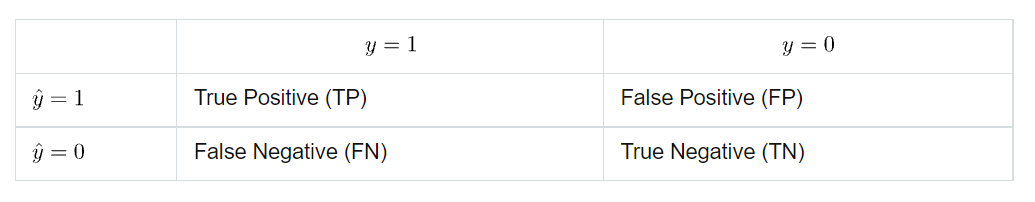
\includegraphics[scale = 1]{errors}

Accuracy - доля правильных ответов алгоритма.

\begin{center}
{$accuracy = \frac{TP + TN}{TP + TN + FP + FN}$}
\end{center}

Recall - полнота, демонстрирует способность алгоритма обнаруживать данный класс в целом.

\begin{center}
{$recall = \frac{TP}{TP + FN}$}
\end{center}

Для оценки качества будет в основном использоваться полнота (recall), а также accuracy. Recall был выбран по следующей причине: в данной задаче false positive не всегда является ошибкой - например, фильм может иметь жанр драмы как неосновной, но это не указано в столбце жанры, а случай false negative грубая ошибка – в датасете помечено, что фильм драма, но к драматичным алгоритм его не отнёс. Лучше всего такую особенность отражает метрика качества recall.
\newpage



\begin{flushleft}
\textbf{\section{Результаты}} % 10
\end{flushleft}

Значения метрик качества:
жанр: драма, число соседей: 221, веса: обратнопропорциональные расстоянию

accuracy: 0.678

recall: 0.860

жанр: комедия, число соседей: 5, веса: экспоненциально убывающие

accuracy: 0.689

recall: 0.581

Качество оказалось не очень высоким, что объясняется сложной структурой признаков. На комедии понизилось качестово recall, это могло быть вызвано меньшим количеством фильмов этого жанра.
\newpage



\begin{flushleft}
\textbf{\section{Листинг кода}} % 11
\end{flushleft}

\small{

    \begin{tcolorbox}[breakable, size=fbox, boxrule=1pt, pad at break*=1mm,colback=cellbackground, colframe=cellborder]
\prompt{In}{incolor}{6}{\boxspacing}
\begin{Verbatim}[commandchars=\\\{\}]
\PY{k+kn}{import} \PY{n+nn}{pandas} \PY{k}{as} \PY{n+nn}{pd}
\PY{k+kn}{import} \PY{n+nn}{numpy} \PY{k}{as} \PY{n+nn}{np}
\PY{k+kn}{import} \PY{n+nn}{matplotlib}\PY{n+nn}{.}\PY{n+nn}{pyplot} \PY{k}{as} \PY{n+nn}{plt}

\PY{k+kn}{from} \PY{n+nn}{sklearn} \PY{k+kn}{import} \PY{n}{neighbors}
\PY{k+kn}{from} \PY{n+nn}{sklearn}\PY{n+nn}{.}\PY{n+nn}{feature\PYZus{}extraction}\PY{n+nn}{.}\PY{n+nn}{text} \PY{k+kn}{import} \PY{n}{TfidfVectorizer}
\PY{k+kn}{from} \PY{n+nn}{sklearn}\PY{n+nn}{.}\PY{n+nn}{metrics} \PY{k+kn}{import} \PY{n}{accuracy\PYZus{}score}\PY{p}{,} \PY{n}{recall\PYZus{}score}
\end{Verbatim}
\end{tcolorbox}

    \hypertarget{ux43eux431ux440ux430ux431ux43eux442ux43aux430-ux434ux430ux43dux43dux44bux445}{%
\subsection{Обработка
данных}\label{ux43eux431ux440ux430ux431ux43eux442ux43aux430-ux434ux430ux43dux43dux44bux445}}

    загружаем датасет

    \begin{tcolorbox}[breakable, size=fbox, boxrule=1pt, pad at break*=1mm,colback=cellbackground, colframe=cellborder]
\prompt{In}{incolor}{7}{\boxspacing}
\begin{Verbatim}[commandchars=\\\{\}]
\PY{n}{movies0} \PY{o}{=} \PY{n}{pd}\PY{o}{.}\PY{n}{read\PYZus{}csv}\PY{p}{(}\PY{l+s+s1}{\PYZsq{}}\PY{l+s+s1}{D:}\PY{l+s+s1}{\PYZbs{}}\PY{l+s+s1}{prac}\PY{l+s+s1}{\PYZbs{}}\PY{l+s+s1}{IMDb movies.csv}\PY{l+s+s1}{\PYZsq{}}\PY{p}{,} \PY{n}{delimiter} \PY{o}{=} \PY{l+s+s1}{\PYZsq{}}\PY{l+s+s1}{,}\PY{l+s+s1}{\PYZsq{}}\PY{p}{,} \PY{n}{low\PYZus{}memory}\PY{o}{=}\PY{k+kc}{False}\PY{p}{)}
\end{Verbatim}
\end{tcolorbox}

    отбираем столбцы, с которыми будем работать

    \begin{tcolorbox}[breakable, size=fbox, boxrule=1pt, pad at break*=1mm,colback=cellbackground, colframe=cellborder]
\prompt{In}{incolor}{8}{\boxspacing}
\begin{Verbatim}[commandchars=\\\{\}]
\PY{n}{movies} \PY{o}{=} \PY{n}{movies0}\PY{p}{[}\PY{p}{[}\PY{l+s+s1}{\PYZsq{}}\PY{l+s+s1}{original\PYZus{}title}\PY{l+s+s1}{\PYZsq{}}\PY{p}{,} \PY{l+s+s1}{\PYZsq{}}\PY{l+s+s1}{description}\PY{l+s+s1}{\PYZsq{}}\PY{p}{,} \PY{l+s+s1}{\PYZsq{}}\PY{l+s+s1}{actors}\PY{l+s+s1}{\PYZsq{}}\PY{p}{,} \PY{l+s+s1}{\PYZsq{}}\PY{l+s+s1}{director}\PY{l+s+s1}{\PYZsq{}}\PY{p}{,} \PY{l+s+s1}{\PYZsq{}}\PY{l+s+s1}{writer}\PY{l+s+s1}{\PYZsq{}}\PY{p}{,} \PY{l+s+s1}{\PYZsq{}}\PY{l+s+s1}{production\PYZus{}company}\PY{l+s+s1}{\PYZsq{}}\PY{p}{,} \PY{l+s+s1}{\PYZsq{}}\PY{l+s+s1}{genre}\PY{l+s+s1}{\PYZsq{}}\PY{p}{]}\PY{p}{]}

\PY{n}{movies}\PY{o}{.}\PY{n}{dropna}\PY{p}{(}\PY{n}{axis}\PY{o}{=}\PY{l+m+mi}{0}\PY{p}{,}\PY{n}{inplace}\PY{o}{=}\PY{k+kc}{True}\PY{p}{)}
\end{Verbatim}
\end{tcolorbox}

    Добавляем столбцы, в которые будем записывать ответы алгоритма

    \begin{tcolorbox}[breakable, size=fbox, boxrule=1pt, pad at break*=1mm,colback=cellbackground, colframe=cellborder]
\prompt{In}{incolor}{9}{\boxspacing}
\begin{Verbatim}[commandchars=\\\{\}]
\PY{n}{movies}\PY{p}{[}\PY{l+s+s1}{\PYZsq{}}\PY{l+s+s1}{drama}\PY{l+s+s1}{\PYZsq{}}\PY{p}{]} \PY{o}{=} \PY{n}{np}\PY{o}{.}\PY{n}{zeros}\PY{p}{(}\PY{n}{movies}\PY{o}{.}\PY{n}{shape}\PY{p}{[}\PY{l+m+mi}{0}\PY{p}{]}\PY{p}{)}
\PY{n}{movies}\PY{p}{[}\PY{l+s+s1}{\PYZsq{}}\PY{l+s+s1}{drama}\PY{l+s+s1}{\PYZsq{}}\PY{p}{]} \PY{o}{=} \PY{n}{np}\PY{o}{.}\PY{n}{where}\PY{p}{(}\PY{p}{(}\PY{n}{movies}\PY{o}{.}\PY{n}{genre}\PY{o}{.}\PY{n}{str}\PY{o}{.}\PY{n}{contains}\PY{p}{(}\PY{l+s+s1}{\PYZsq{}}\PY{l+s+s1}{Drama}\PY{l+s+s1}{\PYZsq{}}\PY{p}{)}\PY{p}{)}\PY{p}{,} \PY{l+m+mi}{1}\PY{p}{,} \PY{n}{movies}\PY{o}{.}\PY{n}{drama}\PY{p}{)}
\PY{n}{movies}\PY{p}{[}\PY{l+s+s1}{\PYZsq{}}\PY{l+s+s1}{comedy}\PY{l+s+s1}{\PYZsq{}}\PY{p}{]} \PY{o}{=} \PY{n}{np}\PY{o}{.}\PY{n}{zeros}\PY{p}{(}\PY{n}{movies}\PY{o}{.}\PY{n}{shape}\PY{p}{[}\PY{l+m+mi}{0}\PY{p}{]}\PY{p}{)}
\PY{n}{movies}\PY{p}{[}\PY{l+s+s1}{\PYZsq{}}\PY{l+s+s1}{comedy}\PY{l+s+s1}{\PYZsq{}}\PY{p}{]} \PY{o}{=} \PY{n}{np}\PY{o}{.}\PY{n}{where}\PY{p}{(}\PY{p}{(}\PY{n}{movies}\PY{o}{.}\PY{n}{genre}\PY{o}{.}\PY{n}{str}\PY{o}{.}\PY{n}{contains}\PY{p}{(}\PY{l+s+s1}{\PYZsq{}}\PY{l+s+s1}{Comedy}\PY{l+s+s1}{\PYZsq{}}\PY{p}{)}\PY{p}{)}\PY{p}{,} \PY{l+m+mi}{1}\PY{p}{,} \PY{n}{movies}\PY{o}{.}\PY{n}{comedy}\PY{p}{)}
\end{Verbatim}
\end{tcolorbox}


   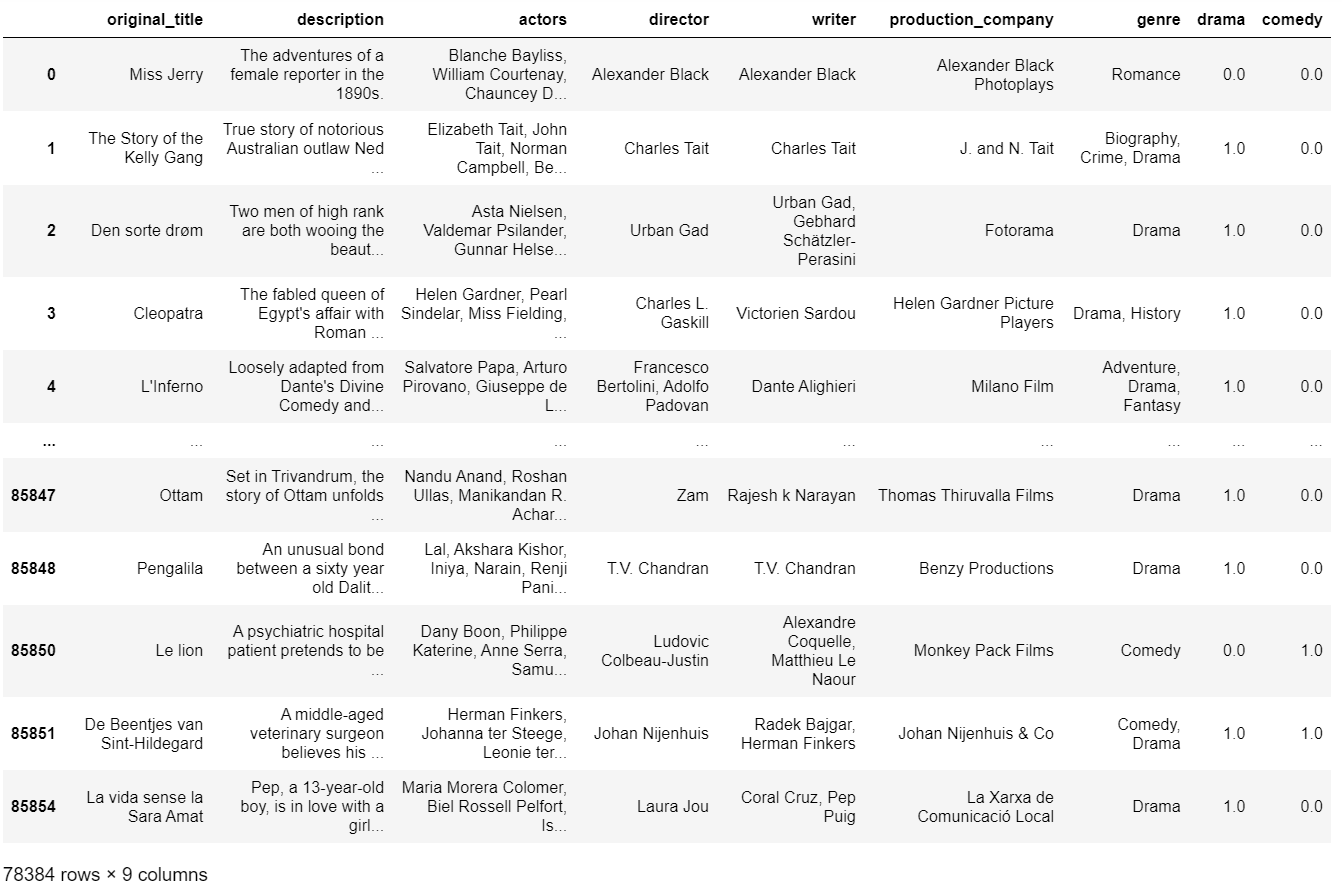
\includegraphics[scale = 1]{1_1}
       

    \hypertarget{ux436ux430ux43dux440-ux434ux440ux430ux43cux430}{%
\subsection{Жанр
драма}\label{ux436ux430ux43dux440-ux434ux440ux430ux43cux430}}


    \begin{tcolorbox}[breakable, size=fbox, boxrule=1pt, pad at break*=1mm,colback=cellbackground, colframe=cellborder]
\prompt{In}{incolor}{37}{\boxspacing}
\begin{Verbatim}[commandchars=\\\{\}]
\PY{k+kn}{from} \PY{n+nn}{sklearn}\PY{n+nn}{.}\PY{n+nn}{model\PYZus{}selection} \PY{k+kn}{import} \PY{n}{train\PYZus{}test\PYZus{}split}
\PY{n}{X} \PY{o}{=} \PY{n}{movies}\PY{p}{[}\PY{l+s+s1}{\PYZsq{}}\PY{l+s+s1}{description}\PY{l+s+s1}{\PYZsq{}}\PY{p}{]} \PY{o}{+} \PY{l+s+s1}{\PYZsq{}}\PY{l+s+s1}{ }\PY{l+s+s1}{\PYZsq{}} \PY{o}{+} \PY{n}{movies}\PY{p}{[}\PY{l+s+s1}{\PYZsq{}}\PY{l+s+s1}{actors}\PY{l+s+s1}{\PYZsq{}}\PY{p}{]} \PY{o}{+} \PY{l+s+s1}{\PYZsq{}}\PY{l+s+s1}{ }\PY{l+s+s1}{\PYZsq{}} \PY{o}{+} \PY{n}{movies}\PY{p}{[}\PY{l+s+s1}{\PYZsq{}}\PY{l+s+s1}{original\PYZus{}title}\PY{l+s+s1}{\PYZsq{}}\PY{p}{]} \PY{o}{+} \PY{l+s+s1}{\PYZsq{}}\PY{l+s+s1}{ }\PY{l+s+s1}{\PYZsq{}} \PY{o}{+} \PY{n}{movies}\PY{p}{[}\PY{l+s+s1}{\PYZsq{}}\PY{l+s+s1}{director}\PY{l+s+s1}{\PYZsq{}}\PY{p}{]} \PY{o}{+} \PY{l+s+s1}{\PYZsq{}}\PY{l+s+s1}{ }\PY{l+s+s1}{\PYZsq{}} \PY{o}{+} \PY{n}{movies}\PY{p}{[}\PY{l+s+s1}{\PYZsq{}}\PY{l+s+s1}{writer}\PY{l+s+s1}{\PYZsq{}}\PY{p}{]} \PY{o}{+} \PY{l+s+s1}{\PYZsq{}}\PY{l+s+s1}{ }\PY{l+s+s1}{\PYZsq{}} \PY{o}{+} \PY{n}{movies}\PY{p}{[}\PY{l+s+s1}{\PYZsq{}}\PY{l+s+s1}{production\PYZus{}company}\PY{l+s+s1}{\PYZsq{}}\PY{p}{]}
\PY{n}{X\PYZus{}train}\PY{p}{,} \PY{n}{X\PYZus{}test}\PY{p}{,} \PY{n}{y\PYZus{}train}\PY{p}{,} \PY{n}{y\PYZus{}test} \PY{o}{=} \PY{n}{train\PYZus{}test\PYZus{}split}\PY{p}{(}\PY{n}{X}\PY{p}{,} \PY{n}{movies}\PY{p}{[}\PY{l+s+s1}{\PYZsq{}}\PY{l+s+s1}{drama}\PY{l+s+s1}{\PYZsq{}}\PY{p}{]}\PY{p}{,}
                                                    \PY{n}{random\PYZus{}state}\PY{o}{=}\PY{l+m+mi}{42}\PY{p}{,} \PY{n}{shuffle}\PY{o}{=}\PY{k+kc}{True}\PY{p}{,} \PY{n}{test\PYZus{}size}\PY{o}{=}\PY{l+m+mf}{0.25}\PY{p}{)}
\PY{n}{X\PYZus{}train} \PY{o}{=} \PY{n}{np}\PY{o}{.}\PY{n}{array}\PY{p}{(}\PY{n}{X\PYZus{}train}\PY{p}{)}
\PY{n}{X\PYZus{}test} \PY{o}{=} \PY{n}{np}\PY{o}{.}\PY{n}{array}\PY{p}{(}\PY{n}{X\PYZus{}test}\PY{p}{)}
\PY{n}{y\PYZus{}train} \PY{o}{=} \PY{n}{np}\PY{o}{.}\PY{n}{array}\PY{p}{(}\PY{n}{y\PYZus{}train}\PY{p}{)}
\PY{n}{y\PYZus{}test} \PY{o}{=} \PY{n}{np}\PY{o}{.}\PY{n}{array}\PY{p}{(}\PY{n}{y\PYZus{}test}\PY{p}{)}

\PY{n+nb}{print}\PY{p}{(}\PY{l+s+sa}{f}\PY{l+s+s1}{\PYZsq{}}\PY{l+s+s1}{пример текста}\PY{l+s+se}{\PYZbs{}n}\PY{l+s+si}{\PYZob{}}\PY{n}{X\PYZus{}train}\PY{p}{[}\PY{l+m+mi}{0}\PY{p}{]}\PY{l+s+si}{\PYZcb{}}\PY{l+s+s1}{\PYZsq{}}\PY{p}{)}
\PY{n+nb}{print}\PY{p}{(}\PY{l+s+sa}{f}\PY{l+s+s1}{\PYZsq{}}\PY{l+s+se}{\PYZbs{}n}\PY{l+s+s1}{размеры выборок: }\PY{l+s+si}{\PYZob{}}\PY{n+nb}{len}\PY{p}{(}\PY{n}{X\PYZus{}train}\PY{p}{)}\PY{p}{,} \PY{n+nb}{len}\PY{p}{(}\PY{n}{X\PYZus{}test}\PY{p}{)}\PY{l+s+si}{\PYZcb{}}\PY{l+s+s1}{\PYZsq{}}\PY{p}{)}
\end{Verbatim}
\end{tcolorbox}

    \begin{Verbatim}[commandchars=\\\{\}]
пример текста
Kyu-sik is a seminary student, who one day falls during a church service,
dropping a precious, pope-blessed relic. As punishment, he and his comic relief
friend Seon-dal are sent away to a {\ldots} Sang-Woo Kwon, Ji-Won Ha, In-kwon Kim,
In-mun Kim, Seon-hwa Kim, Jae-Hyun Cho, Hye-jin Jeon, Hee-soo Kim, Hye-na Kim
Shinbu sueob In-mu Heo In-mu Heo, Eun-kyeong Yun Kihwik Cine

размеры выборок: (58788, 19596)
    \end{Verbatim}

    \hypertarget{ux43eux43fux440ux435ux434ux435ux43bux435ux43dux438ux435-ux444ux443ux43dux43aux446ux438ux439}{%
\subsubsection{Определение
функций}\label{ux43eux43fux440ux435ux434ux435ux43bux435ux43dux438ux435-ux444ux443ux43dux43aux446ux438ux439}}

    \begin{tcolorbox}[breakable, size=fbox, boxrule=1pt, pad at break*=1mm,colback=cellbackground, colframe=cellborder]
\prompt{In}{incolor}{6}{\boxspacing}
\begin{Verbatim}[commandchars=\\\{\}]
\PY{n}{tf\PYZus{}idf} \PY{o}{=} \PY{n}{TfidfVectorizer}\PY{p}{(}\PY{n}{max\PYZus{}df}\PY{o}{=}\PY{l+m+mf}{0.8}\PY{p}{,} \PY{n}{min\PYZus{}df}\PY{o}{=}\PY{l+m+mi}{10}\PY{p}{,} \PY{n}{stop\PYZus{}words}\PY{o}{=}\PY{l+s+s1}{\PYZsq{}}\PY{l+s+s1}{english}\PY{l+s+s1}{\PYZsq{}}\PY{p}{)}
\end{Verbatim}
\end{tcolorbox}

    Функция, считающая качество обучения на кросс валидации.

    \begin{tcolorbox}[breakable, size=fbox, boxrule=1pt, pad at break*=1mm,colback=cellbackground, colframe=cellborder]
\prompt{In}{incolor}{7}{\boxspacing}
\begin{Verbatim}[commandchars=\\\{\}]
\PY{k}{def} \PY{n+nf}{cv\PYZus{}score}\PY{p}{(}\PY{n}{X}\PY{p}{,} \PY{n}{y}\PY{p}{,} \PY{n}{parameters}\PY{p}{,} \PY{n}{folds}\PY{p}{,} \PY{n}{knn\PYZus{}class}\PY{p}{)}\PY{p}{:}
    \PY{n}{ans} \PY{o}{=} \PY{p}{[}\PY{p}{]}
    \PY{n}{scaler} \PY{o}{=} \PY{n}{TfidfVectorizer}\PY{p}{(}\PY{n}{max\PYZus{}df}\PY{o}{=}\PY{l+m+mf}{0.8}\PY{p}{,} \PY{n}{min\PYZus{}df}\PY{o}{=}\PY{l+m+mi}{10}\PY{p}{,} \PY{n}{stop\PYZus{}words}\PY{o}{=}\PY{l+s+s1}{\PYZsq{}}\PY{l+s+s1}{english}\PY{l+s+s1}{\PYZsq{}}\PY{p}{)}
    \PY{k}{for} \PY{n}{sc} \PY{o+ow}{in} \PY{n}{parameters}\PY{p}{[}\PY{l+s+s1}{\PYZsq{}}\PY{l+s+s1}{scores}\PY{l+s+s1}{\PYZsq{}}\PY{p}{]}\PY{p}{:}
        \PY{n}{ans}\PY{o}{.}\PY{n}{append}\PY{p}{(}\PY{p}{\PYZob{}}\PY{p}{\PYZcb{}}\PY{p}{)}
        \PY{k}{for} \PY{n}{n} \PY{o+ow}{in} \PY{n}{parameters}\PY{p}{[}\PY{l+s+s1}{\PYZsq{}}\PY{l+s+s1}{n\PYZus{}neighbors}\PY{l+s+s1}{\PYZsq{}}\PY{p}{]}\PY{p}{:}
            \PY{k}{for} \PY{n}{w} \PY{o+ow}{in} \PY{n}{parameters}\PY{p}{[}\PY{l+s+s1}{\PYZsq{}}\PY{l+s+s1}{weights}\PY{l+s+s1}{\PYZsq{}}\PY{p}{]}\PY{p}{:}
                \PY{n}{neigh} \PY{o}{=} \PY{n}{knn\PYZus{}class}\PY{p}{(}\PY{n}{n\PYZus{}neighbors}\PY{o}{=}\PY{n}{n}\PY{p}{,} \PY{n}{metric}\PY{o}{=}\PY{l+s+s1}{\PYZsq{}}\PY{l+s+s1}{cosine}\PY{l+s+s1}{\PYZsq{}}\PY{p}{,} \PY{n}{weights}\PY{o}{=}\PY{n}{w}\PY{p}{[}\PY{l+m+mi}{1}\PY{p}{]}\PY{p}{)}
                \PY{n}{i} \PY{o}{=} \PY{n}{parameters}\PY{p}{[}\PY{l+s+s1}{\PYZsq{}}\PY{l+s+s1}{scores}\PY{l+s+s1}{\PYZsq{}}\PY{p}{]}\PY{o}{.}\PY{n}{index}\PY{p}{(}\PY{n}{sc}\PY{p}{)}
                \PY{n}{ans}\PY{p}{[}\PY{n}{i}\PY{p}{]}\PY{p}{[}\PY{p}{(}\PY{n}{n}\PY{p}{,} \PY{n}{w}\PY{p}{[}\PY{l+m+mi}{0}\PY{p}{]}\PY{p}{)}\PY{p}{]} \PY{o}{=} \PY{l+m+mi}{0}
                \PY{k}{for} \PY{n}{f} \PY{o+ow}{in} \PY{n}{folds}\PY{p}{:}
                    \PY{n}{scaler}\PY{o}{.}\PY{n}{fit}\PY{p}{(}\PY{n}{X}\PY{p}{[}\PY{n}{f}\PY{p}{[}\PY{l+m+mi}{0}\PY{p}{]}\PY{p}{]}\PY{p}{)}
                    \PY{n}{X\PYZus{}train} \PY{o}{=} \PY{n}{scaler}\PY{o}{.}\PY{n}{transform}\PY{p}{(}\PY{n}{X}\PY{p}{[}\PY{n}{f}\PY{p}{[}\PY{l+m+mi}{0}\PY{p}{]}\PY{p}{]}\PY{p}{)}
                    \PY{n}{X\PYZus{}test} \PY{o}{=} \PY{n}{scaler}\PY{o}{.}\PY{n}{transform}\PY{p}{(}\PY{n}{X}\PY{p}{[}\PY{n}{f}\PY{p}{[}\PY{l+m+mi}{1}\PY{p}{]}\PY{p}{]}\PY{p}{)}
                    \PY{n}{neigh}\PY{o}{.}\PY{n}{fit}\PY{p}{(}\PY{n}{X\PYZus{}train}\PY{p}{,} \PY{n}{y}\PY{p}{[}\PY{n}{f}\PY{p}{[}\PY{l+m+mi}{0}\PY{p}{]}\PY{p}{]}\PY{p}{)}
                    \PY{n}{ans}\PY{p}{[}\PY{n}{i}\PY{p}{]}\PY{p}{[}\PY{p}{(}\PY{n}{n}\PY{p}{,} \PY{n}{w}\PY{p}{[}\PY{l+m+mi}{0}\PY{p}{]}\PY{p}{)}\PY{p}{]} \PY{o}{+}\PY{o}{=} \PY{n}{sc}\PY{p}{(}\PY{n}{y}\PY{p}{[}\PY{n}{f}\PY{p}{[}\PY{l+m+mi}{1}\PY{p}{]}\PY{p}{]}\PY{p}{,} \PY{n}{neigh}\PY{o}{.}\PY{n}{predict}\PY{p}{(}\PY{n}{X\PYZus{}test}\PY{p}{)}\PY{p}{)}
                \PY{n}{ans}\PY{p}{[}\PY{n}{i}\PY{p}{]}\PY{p}{[}\PY{p}{(}\PY{n}{n}\PY{p}{,} \PY{n}{w}\PY{p}{[}\PY{l+m+mi}{0}\PY{p}{]}\PY{p}{)}\PY{p}{]} \PY{o}{/}\PY{o}{=} \PY{n+nb}{len}\PY{p}{(}\PY{n}{folds}\PY{p}{)}
    \PY{k}{return} \PY{n}{ans}
\end{Verbatim}
\end{tcolorbox}

    Функция, разбивающая обучающую выборку на блоки (folds) для кросс
валидации

    \begin{tcolorbox}[breakable, size=fbox, boxrule=1pt, pad at break*=1mm,colback=cellbackground, colframe=cellborder]
\prompt{In}{incolor}{8}{\boxspacing}
\begin{Verbatim}[commandchars=\\\{\}]
\PY{k}{def} \PY{n+nf}{fold\PYZus{}split}\PY{p}{(}\PY{n}{num\PYZus{}objects}\PY{p}{,} \PY{n}{num\PYZus{}folds}\PY{p}{)}\PY{p}{:}
    \PY{n}{fold\PYZus{}size} \PY{o}{=} \PY{n}{num\PYZus{}objects} \PY{o}{/}\PY{o}{/} \PY{n}{num\PYZus{}folds}
    \PY{n}{flag} \PY{o}{=} \PY{n}{num\PYZus{}objects} \PY{o}{\PYZpc{}} \PY{n}{num\PYZus{}folds}
    \PY{n}{ans} \PY{o}{=} \PY{n+nb}{list}\PY{p}{(}\PY{p}{)}
    \PY{k}{for} \PY{n}{i} \PY{o+ow}{in} \PY{n+nb}{range}\PY{p}{(}\PY{n}{num\PYZus{}folds}\PY{p}{)}\PY{p}{:}
        \PY{n}{x} \PY{o}{=} \PY{n}{np}\PY{o}{.}\PY{n}{arange}\PY{p}{(}\PY{n}{num\PYZus{}objects}\PY{p}{)}
        \PY{n}{mask1} \PY{o}{=} \PY{p}{(}\PY{n}{x} \PY{o}{\PYZgt{}}\PY{o}{=} \PY{p}{(}\PY{n}{i} \PY{o}{+} \PY{l+m+mi}{1}\PY{p}{)} \PY{o}{*} \PY{n}{fold\PYZus{}size}\PY{p}{)} \PY{o}{|} \PY{p}{(}\PY{n}{x} \PY{o}{\PYZlt{}} \PY{n}{i} \PY{o}{*} \PY{n}{fold\PYZus{}size}\PY{p}{)}
        \PY{n}{mask2} \PY{o}{=} \PY{p}{(}\PY{n}{x} \PY{o}{\PYZlt{}} \PY{p}{(}\PY{n}{i} \PY{o}{+} \PY{l+m+mi}{1}\PY{p}{)} \PY{o}{*} \PY{n}{fold\PYZus{}size}\PY{p}{)} \PY{o}{\PYZam{}} \PY{p}{(}\PY{n}{x} \PY{o}{\PYZgt{}}\PY{o}{=} \PY{n}{i} \PY{o}{*} \PY{n}{fold\PYZus{}size}\PY{p}{)}
        \PY{k}{if} \PY{n}{flag} \PY{o+ow}{and} \PY{n}{i} \PY{o}{==} \PY{n}{num\PYZus{}folds} \PY{o}{\PYZhy{}} \PY{l+m+mi}{1}\PY{p}{:}
            \PY{n}{ans}\PY{o}{.}\PY{n}{append}\PY{p}{(}\PY{p}{(}\PY{n}{x}\PY{p}{[}\PY{n}{x} \PY{o}{\PYZlt{}} \PY{n}{i} \PY{o}{*} \PY{n}{fold\PYZus{}size}\PY{p}{]}\PY{p}{,} \PY{n}{x}\PY{p}{[}\PY{n}{x} \PY{o}{\PYZgt{}}\PY{o}{=} \PY{n}{i} \PY{o}{*} \PY{n}{fold\PYZus{}size}\PY{p}{]}\PY{p}{)}\PY{p}{)}
            \PY{k}{break}
        \PY{n}{ans}\PY{o}{.}\PY{n}{append}\PY{p}{(}\PY{p}{(}\PY{n}{x}\PY{p}{[}\PY{n}{mask1}\PY{p}{]}\PY{p}{,} \PY{n}{x}\PY{p}{[}\PY{n}{mask2}\PY{p}{]}\PY{p}{)}\PY{p}{)}
    \PY{k}{return} \PY{n}{ans}
\end{Verbatim}
\end{tcolorbox}

    реализация линейно и экспоненциально убывающих весов

    \begin{tcolorbox}[breakable, size=fbox, boxrule=1pt, pad at break*=1mm,colback=cellbackground, colframe=cellborder]
\prompt{In}{incolor}{23}{\boxspacing}
\begin{Verbatim}[commandchars=\\\{\}]
\PY{k}{def} \PY{n+nf}{linear}\PY{p}{(}\PY{n}{distances}\PY{p}{:} \PY{n}{np}\PY{o}{.}\PY{n}{array}\PY{p}{)}\PY{o}{\PYZhy{}}\PY{o}{\PYZgt{}}\PY{n}{np}\PY{o}{.}\PY{n}{array}\PY{p}{:}
    \PY{n}{weights}\PY{p}{:} \PY{n}{np}\PY{o}{.}\PY{n}{array} \PY{o}{=} \PY{n}{np}\PY{o}{.}\PY{n}{array}\PY{p}{(}\PY{n}{np}\PY{o}{.}\PY{n}{full}\PY{p}{(}\PY{n}{distances}\PY{o}{.}\PY{n}{shape}\PY{p}{,} \PY{l+m+mi}{0}\PY{p}{)}\PY{p}{,} \PY{n}{dtype}\PY{o}{=}\PY{l+s+s1}{\PYZsq{}}\PY{l+s+s1}{float}\PY{l+s+s1}{\PYZsq{}}\PY{p}{)}
    \PY{n}{n} \PY{o}{=} \PY{n}{distances}\PY{o}{.}\PY{n}{shape}\PY{p}{[}\PY{l+m+mi}{1}\PY{p}{]}
    \PY{n}{weights}\PY{p}{[}\PY{p}{:}\PY{p}{]} \PY{o}{=} \PY{n}{np}\PY{o}{.}\PY{n}{arange}\PY{p}{(}\PY{l+m+mf}{1.0}\PY{p}{,} \PY{l+m+mi}{0}\PY{p}{,} \PY{o}{\PYZhy{}}\PY{l+m+mi}{1} \PY{o}{/} \PY{n}{n}\PY{p}{)}
    \PY{k}{return} \PY{n}{weights}

\PY{k}{def} \PY{n+nf}{my\PYZus{}exp}\PY{p}{(}\PY{n}{distances}\PY{p}{:} \PY{n}{np}\PY{o}{.}\PY{n}{array}\PY{p}{)}\PY{o}{\PYZhy{}}\PY{o}{\PYZgt{}}\PY{n}{np}\PY{o}{.}\PY{n}{array}\PY{p}{:}
    \PY{n}{weights}\PY{p}{:} \PY{n}{np}\PY{o}{.}\PY{n}{array} \PY{o}{=} \PY{n}{np}\PY{o}{.}\PY{n}{array}\PY{p}{(}\PY{n}{np}\PY{o}{.}\PY{n}{full}\PY{p}{(}\PY{n}{distances}\PY{o}{.}\PY{n}{shape}\PY{p}{,} \PY{l+m+mi}{0}\PY{p}{)}\PY{p}{,} \PY{n}{dtype}\PY{o}{=}\PY{l+s+s1}{\PYZsq{}}\PY{l+s+s1}{float}\PY{l+s+s1}{\PYZsq{}}\PY{p}{)}
    \PY{n}{n} \PY{o}{=} \PY{n}{distances}\PY{o}{.}\PY{n}{shape}\PY{p}{[}\PY{l+m+mi}{1}\PY{p}{]}
    \PY{n}{weights}\PY{p}{[}\PY{p}{:}\PY{p}{]} \PY{o}{=} \PY{n}{np}\PY{o}{.}\PY{n}{geomspace}\PY{p}{(}\PY{l+m+mi}{1}\PY{p}{,} \PY{p}{(}\PY{l+m+mi}{1}\PY{o}{/}\PY{l+m+mi}{2}\PY{p}{)} \PY{o}{*}\PY{o}{*} \PY{p}{(}\PY{n}{n} \PY{o}{\PYZhy{}} \PY{l+m+mi}{1}\PY{p}{)}\PY{p}{,} \PY{n}{n}\PY{p}{)}
    \PY{k}{return} \PY{n}{weights}
\end{Verbatim}
\end{tcolorbox}

    \hypertarget{ux432ux44bux431ux43eux440-ux432ux435ux441ux430-ux44dux442ux430ux43f-0}{%
\subsubsection{Выбор веса (этап
0)}\label{ux432ux44bux431ux43eux440-ux432ux435ux441ux430-ux44dux442ux430ux43f-0}}

    Первый набор параметров

    \begin{tcolorbox}[breakable, size=fbox, boxrule=1pt, pad at break*=1mm,colback=cellbackground, colframe=cellborder]
\prompt{In}{incolor}{11}{\boxspacing}
\begin{Verbatim}[commandchars=\\\{\}]
\PY{n}{par0} \PY{o}{=} \PY{p}{\PYZob{}}
    \PY{l+s+s1}{\PYZsq{}}\PY{l+s+s1}{n\PYZus{}neighbors}\PY{l+s+s1}{\PYZsq{}}\PY{p}{:} \PY{p}{[}\PY{n}{i} \PY{k}{for} \PY{n}{i} \PY{o+ow}{in} \PY{n+nb}{range}\PY{p}{(}\PY{l+m+mi}{1}\PY{p}{,} \PY{l+m+mi}{11}\PY{p}{)}\PY{p}{]}\PY{p}{,}
    \PY{l+s+s1}{\PYZsq{}}\PY{l+s+s1}{weights}\PY{l+s+s1}{\PYZsq{}}\PY{p}{:} \PY{p}{[}\PY{p}{(}\PY{l+s+s1}{\PYZsq{}}\PY{l+s+s1}{uniform}\PY{l+s+s1}{\PYZsq{}}\PY{p}{,} \PY{l+s+s1}{\PYZsq{}}\PY{l+s+s1}{uniform}\PY{l+s+s1}{\PYZsq{}}\PY{p}{)}\PY{p}{,} \PY{p}{(}\PY{l+s+s1}{\PYZsq{}}\PY{l+s+s1}{linear}\PY{l+s+s1}{\PYZsq{}}\PY{p}{,} \PY{n}{linear}\PY{p}{)}\PY{p}{,} \PY{p}{(}\PY{l+s+s1}{\PYZsq{}}\PY{l+s+s1}{my\PYZus{}exp}\PY{l+s+s1}{\PYZsq{}}\PY{p}{,} \PY{n}{my\PYZus{}exp}\PY{p}{)}\PY{p}{,} \PY{p}{(}\PY{l+s+s1}{\PYZsq{}}\PY{l+s+s1}{distance}\PY{l+s+s1}{\PYZsq{}}\PY{p}{,} \PY{l+s+s1}{\PYZsq{}}\PY{l+s+s1}{distance}\PY{l+s+s1}{\PYZsq{}}\PY{p}{)}\PY{p}{]}\PY{p}{,}
    \PY{l+s+s1}{\PYZsq{}}\PY{l+s+s1}{scores}\PY{l+s+s1}{\PYZsq{}}\PY{p}{:} \PY{p}{[}\PY{n}{recall\PYZus{}score}\PY{p}{]}
\PY{p}{\PYZcb{}}
\end{Verbatim}
\end{tcolorbox}

    \begin{tcolorbox}[breakable, size=fbox, boxrule=1pt, pad at break*=1mm,colback=cellbackground, colframe=cellborder]
\prompt{In}{incolor}{12}{\boxspacing}
\begin{Verbatim}[commandchars=\\\{\}]
\PY{n}{folds0} \PY{o}{=} \PY{n}{fold\PYZus{}split}\PY{p}{(}\PY{n+nb}{len}\PY{p}{(}\PY{n}{y\PYZus{}train}\PY{p}{)}\PY{p}{,} \PY{l+m+mi}{4}\PY{p}{)}
\PY{n}{score\PYZus{}train0} \PY{o}{=} \PY{n}{cv\PYZus{}score}\PY{p}{(}\PY{n}{X\PYZus{}train}\PY{p}{,} \PY{n}{y\PYZus{}train}\PY{p}{,} \PY{n}{par0}\PY{p}{,} \PY{n}{folds0}\PY{p}{,} \PY{n}{neighbors}\PY{o}{.}\PY{n}{KNeighborsClassifier}\PY{p}{)}
\end{Verbatim}
\end{tcolorbox}

    Посчитаем, где в среднем качество лучше

    \begin{tcolorbox}[breakable, size=fbox, boxrule=1pt, pad at break*=1mm,colback=cellbackground, colframe=cellborder]
\prompt{In}{incolor}{15}{\boxspacing}
\begin{Verbatim}[commandchars=\\\{\}]
\PY{n}{n} \PY{o}{=} \PY{l+m+mi}{10}
\PY{n}{score\PYZus{}weights} \PY{o}{=} \PY{p}{\PYZob{}}\PY{l+s+s1}{\PYZsq{}}\PY{l+s+s1}{uniform}\PY{l+s+s1}{\PYZsq{}}\PY{p}{:} \PY{l+m+mi}{0}\PY{p}{,} \PY{l+s+s1}{\PYZsq{}}\PY{l+s+s1}{linear}\PY{l+s+s1}{\PYZsq{}}\PY{p}{:} \PY{l+m+mi}{0}\PY{p}{,} \PY{l+s+s1}{\PYZsq{}}\PY{l+s+s1}{my\PYZus{}exp}\PY{l+s+s1}{\PYZsq{}}\PY{p}{:} \PY{l+m+mi}{0}\PY{p}{,} \PY{l+s+s1}{\PYZsq{}}\PY{l+s+s1}{distance}\PY{l+s+s1}{\PYZsq{}}\PY{p}{:} \PY{l+m+mi}{0}\PY{p}{\PYZcb{}}
\PY{k}{for} \PY{n}{i} \PY{o+ow}{in} \PY{n}{score\PYZus{}train0}\PY{p}{[}\PY{l+m+mi}{0}\PY{p}{]}\PY{o}{.}\PY{n}{keys}\PY{p}{(}\PY{p}{)}\PY{p}{:}
    \PY{n}{score\PYZus{}weights}\PY{p}{[}\PY{n}{i}\PY{p}{[}\PY{l+m+mi}{1}\PY{p}{]}\PY{p}{]} \PY{o}{+}\PY{o}{=} \PY{n}{score\PYZus{}train0}\PY{p}{[}\PY{l+m+mi}{0}\PY{p}{]}\PY{p}{[}\PY{n}{i}\PY{p}{]} \PY{o}{/} \PY{n}{n}
\PY{n}{score\PYZus{}weights}
\end{Verbatim}
\end{tcolorbox}

            \begin{tcolorbox}[breakable, size=fbox, boxrule=.5pt, pad at break*=1mm, opacityfill=0]
\prompt{Out}{outcolor}{15}{\boxspacing}
\begin{Verbatim}[commandchars=\\\{\}]
\{'uniform': 0.6434384348115793,
 'linear': 0.6953085178688904,
 'my\_exp': 0.6605275499731177,
 'distance': 0.7065966666916362\}
\end{Verbatim}
\end{tcolorbox}
        
    качество в среднем лучше на весах по расстоянию

    \hypertarget{ux432ux44bux431ux43eux440-ux43aux43eux43bux438ux447ux435ux441ux442ux432ux430-ux441ux43eux441ux435ux434ux435ux439-ux44dux442ux430ux43f-1}{%
\subsubsection{Выбор количества соседей (этап
1)}\label{ux432ux44bux431ux43eux440-ux43aux43eux43bux438ux447ux435ux441ux442ux432ux430-ux441ux43eux441ux435ux434ux435ux439-ux44dux442ux430ux43f-1}}

    \begin{tcolorbox}[breakable, size=fbox, boxrule=1pt, pad at break*=1mm,colback=cellbackground, colframe=cellborder]
\prompt{In}{incolor}{21}{\boxspacing}
\begin{Verbatim}[commandchars=\\\{\}]
\PY{n}{tf\PYZus{}idf} \PY{o}{=} \PY{n}{TfidfVectorizer}\PY{p}{(}\PY{n}{max\PYZus{}df}\PY{o}{=}\PY{l+m+mf}{0.8}\PY{p}{,} \PY{n}{min\PYZus{}df}\PY{o}{=}\PY{l+m+mi}{10}\PY{p}{,} \PY{n}{stop\PYZus{}words}\PY{o}{=}\PY{l+s+s1}{\PYZsq{}}\PY{l+s+s1}{english}\PY{l+s+s1}{\PYZsq{}}\PY{p}{)}
\PY{n}{par1} \PY{o}{=} \PY{p}{\PYZob{}}
    \PY{l+s+s1}{\PYZsq{}}\PY{l+s+s1}{n\PYZus{}neighbors}\PY{l+s+s1}{\PYZsq{}}\PY{p}{:} \PY{p}{[}\PY{n}{i} \PY{k}{for} \PY{n}{i} \PY{o+ow}{in} \PY{n+nb}{range}\PY{p}{(}\PY{l+m+mi}{1}\PY{p}{,} \PY{l+m+mi}{200}\PY{p}{,} \PY{l+m+mi}{10}\PY{p}{)}\PY{p}{]}\PY{p}{,}
    \PY{l+s+s1}{\PYZsq{}}\PY{l+s+s1}{weights}\PY{l+s+s1}{\PYZsq{}}\PY{p}{:} \PY{p}{[}\PY{p}{(}\PY{l+s+s1}{\PYZsq{}}\PY{l+s+s1}{distance}\PY{l+s+s1}{\PYZsq{}}\PY{p}{,} \PY{l+s+s1}{\PYZsq{}}\PY{l+s+s1}{distance}\PY{l+s+s1}{\PYZsq{}}\PY{p}{)}\PY{p}{]}\PY{p}{,}
    \PY{l+s+s1}{\PYZsq{}}\PY{l+s+s1}{scores}\PY{l+s+s1}{\PYZsq{}}\PY{p}{:} \PY{p}{[}\PY{n}{recall\PYZus{}score}\PY{p}{,} \PY{n}{accuracy\PYZus{}score}\PY{p}{]}
\PY{p}{\PYZcb{}}
\end{Verbatim}
\end{tcolorbox}

    \begin{tcolorbox}[breakable, size=fbox, boxrule=1pt, pad at break*=1mm,colback=cellbackground, colframe=cellborder]
\prompt{In}{incolor}{22}{\boxspacing}
\begin{Verbatim}[commandchars=\\\{\}]
\PY{n}{folds1} \PY{o}{=} \PY{n}{fold\PYZus{}split}\PY{p}{(}\PY{n+nb}{len}\PY{p}{(}\PY{n}{y\PYZus{}train}\PY{p}{)}\PY{p}{,} \PY{l+m+mi}{4}\PY{p}{)}
\PY{n}{score\PYZus{}train1} \PY{o}{=} \PY{n}{cv\PYZus{}score}\PY{p}{(}\PY{n}{X\PYZus{}train}\PY{p}{,} \PY{n}{y\PYZus{}train}\PY{p}{,} \PY{n}{par1}\PY{p}{,} \PY{n}{folds1}\PY{p}{,} \PY{n}{neighbors}\PY{o}{.}\PY{n}{KNeighborsClassifier}\PY{p}{)}
\end{Verbatim}
\end{tcolorbox}

    \begin{tcolorbox}[breakable, size=fbox, boxrule=1pt, pad at break*=1mm,colback=cellbackground, colframe=cellborder]
\prompt{In}{incolor}{23}{\boxspacing}
\begin{Verbatim}[commandchars=\\\{\}]
\PY{n}{plt}\PY{o}{.}\PY{n}{plot}\PY{p}{(}\PY{n}{par1}\PY{p}{[}\PY{l+s+s1}{\PYZsq{}}\PY{l+s+s1}{n\PYZus{}neighbors}\PY{l+s+s1}{\PYZsq{}}\PY{p}{]}\PY{p}{,} \PY{n+nb}{list}\PY{p}{(}\PY{n}{score\PYZus{}train1}\PY{p}{[}\PY{l+m+mi}{0}\PY{p}{]}\PY{o}{.}\PY{n}{values}\PY{p}{(}\PY{p}{)}\PY{p}{)}\PY{p}{)}
\PY{n}{plt}\PY{o}{.}\PY{n}{plot}\PY{p}{(}\PY{n}{par1}\PY{p}{[}\PY{l+s+s1}{\PYZsq{}}\PY{l+s+s1}{n\PYZus{}neighbors}\PY{l+s+s1}{\PYZsq{}}\PY{p}{]}\PY{p}{,} \PY{n+nb}{list}\PY{p}{(}\PY{n}{score\PYZus{}train1}\PY{p}{[}\PY{l+m+mi}{1}\PY{p}{]}\PY{o}{.}\PY{n}{values}\PY{p}{(}\PY{p}{)}\PY{p}{)}\PY{p}{)}
\PY{n}{plt}\PY{o}{.}\PY{n}{xlabel}\PY{p}{(}\PY{l+s+s2}{\PYZdq{}}\PY{l+s+s2}{neighbors}\PY{l+s+s2}{\PYZdq{}}\PY{p}{)}
\PY{n}{plt}\PY{o}{.}\PY{n}{ylabel}\PY{p}{(}\PY{l+s+s2}{\PYZdq{}}\PY{l+s+s2}{score}\PY{l+s+s2}{\PYZdq{}}\PY{p}{)}
\end{Verbatim}
\end{tcolorbox}

            \begin{tcolorbox}[breakable, size=fbox, boxrule=.5pt, pad at break*=1mm, opacityfill=0]
\prompt{Out}{outcolor}{23}{\boxspacing}
\begin{Verbatim}[commandchars=\\\{\}]
Text(0, 0.5, 'score')
\end{Verbatim}
\end{tcolorbox}
        
    \begin{center}
    \adjustimage{max size={0.9\linewidth}{0.9\paperheight}}{output_31_1.png}
    \end{center}
    { \hspace*{\fill} \\}
    
    посмотрим на всякий случай изменение качества и на дальше: на 200-400
соседях

    \begin{tcolorbox}[breakable, size=fbox, boxrule=1pt, pad at break*=1mm,colback=cellbackground, colframe=cellborder]
\prompt{In}{incolor}{16}{\boxspacing}
\begin{Verbatim}[commandchars=\\\{\}]
\PY{n}{tf\PYZus{}idf} \PY{o}{=} \PY{n}{TfidfVectorizer}\PY{p}{(}\PY{n}{max\PYZus{}df}\PY{o}{=}\PY{l+m+mf}{0.8}\PY{p}{,} \PY{n}{min\PYZus{}df}\PY{o}{=}\PY{l+m+mi}{10}\PY{p}{,} \PY{n}{stop\PYZus{}words}\PY{o}{=}\PY{l+s+s1}{\PYZsq{}}\PY{l+s+s1}{english}\PY{l+s+s1}{\PYZsq{}}\PY{p}{)}
\PY{n}{par1\PYZus{}2} \PY{o}{=} \PY{p}{\PYZob{}}
    \PY{l+s+s1}{\PYZsq{}}\PY{l+s+s1}{n\PYZus{}neighbors}\PY{l+s+s1}{\PYZsq{}}\PY{p}{:} \PY{p}{[}\PY{n}{i} \PY{k}{for} \PY{n}{i} \PY{o+ow}{in} \PY{n+nb}{range}\PY{p}{(}\PY{l+m+mi}{201}\PY{p}{,} \PY{l+m+mi}{402}\PY{p}{,} \PY{l+m+mi}{10}\PY{p}{)}\PY{p}{]}\PY{p}{,}
    \PY{l+s+s1}{\PYZsq{}}\PY{l+s+s1}{weights}\PY{l+s+s1}{\PYZsq{}}\PY{p}{:} \PY{p}{[}\PY{p}{(}\PY{l+s+s1}{\PYZsq{}}\PY{l+s+s1}{distance}\PY{l+s+s1}{\PYZsq{}}\PY{p}{,} \PY{l+s+s1}{\PYZsq{}}\PY{l+s+s1}{distance}\PY{l+s+s1}{\PYZsq{}}\PY{p}{)}\PY{p}{]}\PY{p}{,}
    \PY{l+s+s1}{\PYZsq{}}\PY{l+s+s1}{scores}\PY{l+s+s1}{\PYZsq{}}\PY{p}{:} \PY{p}{[}\PY{n}{recall\PYZus{}score}\PY{p}{,} \PY{n}{accuracy\PYZus{}score}\PY{p}{]}
\PY{p}{\PYZcb{}}
\end{Verbatim}
\end{tcolorbox}

    \begin{tcolorbox}[breakable, size=fbox, boxrule=1pt, pad at break*=1mm,colback=cellbackground, colframe=cellborder]
\prompt{In}{incolor}{17}{\boxspacing}
\begin{Verbatim}[commandchars=\\\{\}]
\PY{n}{folds1} \PY{o}{=} \PY{n}{fold\PYZus{}split}\PY{p}{(}\PY{n+nb}{len}\PY{p}{(}\PY{n}{y\PYZus{}train}\PY{p}{)}\PY{p}{,} \PY{l+m+mi}{4}\PY{p}{)}
\PY{n}{score\PYZus{}train1\PYZus{}2} \PY{o}{=} \PY{n}{cv\PYZus{}score}\PY{p}{(}\PY{n}{X\PYZus{}train}\PY{p}{,} \PY{n}{y\PYZus{}train}\PY{p}{,} \PY{n}{par1\PYZus{}2}\PY{p}{,} \PY{n}{folds1}\PY{p}{,} \PY{n}{neighbors}\PY{o}{.}\PY{n}{KNeighborsClassifier}\PY{p}{)}
\end{Verbatim}
\end{tcolorbox}

    \begin{tcolorbox}[breakable, size=fbox, boxrule=1pt, pad at break*=1mm,colback=cellbackground, colframe=cellborder]
\prompt{In}{incolor}{18}{\boxspacing}
\begin{Verbatim}[commandchars=\\\{\}]
\PY{n}{plt}\PY{o}{.}\PY{n}{plot}\PY{p}{(}\PY{n}{par1\PYZus{}2}\PY{p}{[}\PY{l+s+s1}{\PYZsq{}}\PY{l+s+s1}{n\PYZus{}neighbors}\PY{l+s+s1}{\PYZsq{}}\PY{p}{]}\PY{p}{,} \PY{n+nb}{list}\PY{p}{(}\PY{n}{score\PYZus{}train1\PYZus{}2}\PY{p}{[}\PY{l+m+mi}{0}\PY{p}{]}\PY{o}{.}\PY{n}{values}\PY{p}{(}\PY{p}{)}\PY{p}{)}\PY{p}{)}
\PY{n}{plt}\PY{o}{.}\PY{n}{plot}\PY{p}{(}\PY{n}{par1\PYZus{}2}\PY{p}{[}\PY{l+s+s1}{\PYZsq{}}\PY{l+s+s1}{n\PYZus{}neighbors}\PY{l+s+s1}{\PYZsq{}}\PY{p}{]}\PY{p}{,} \PY{n+nb}{list}\PY{p}{(}\PY{n}{score\PYZus{}train1\PYZus{}2}\PY{p}{[}\PY{l+m+mi}{1}\PY{p}{]}\PY{o}{.}\PY{n}{values}\PY{p}{(}\PY{p}{)}\PY{p}{)}\PY{p}{)}
\PY{n}{plt}\PY{o}{.}\PY{n}{xlabel}\PY{p}{(}\PY{l+s+s2}{\PYZdq{}}\PY{l+s+s2}{neighbors}\PY{l+s+s2}{\PYZdq{}}\PY{p}{)}
\PY{n}{plt}\PY{o}{.}\PY{n}{ylabel}\PY{p}{(}\PY{l+s+s2}{\PYZdq{}}\PY{l+s+s2}{score}\PY{l+s+s2}{\PYZdq{}}\PY{p}{)}
\end{Verbatim}
\end{tcolorbox}

            \begin{tcolorbox}[breakable, size=fbox, boxrule=.5pt, pad at break*=1mm, opacityfill=0]
\prompt{Out}{outcolor}{18}{\boxspacing}
\begin{Verbatim}[commandchars=\\\{\}]
Text(0, 0.5, 'score')
\end{Verbatim}
\end{tcolorbox}
        
    \begin{center}
    \adjustimage{max size={0.9\linewidth}{0.9\paperheight}}{output_35_1.png}
    \end{center}
    { \hspace*{\fill} \\}
    
    recall немного растёт, accuracy не меняется

    \begin{tcolorbox}[breakable, size=fbox, boxrule=1pt, pad at break*=1mm,colback=cellbackground, colframe=cellborder]
\prompt{In}{incolor}{25}{\boxspacing}
\begin{Verbatim}[commandchars=\\\{\}]
\PY{k}{for} \PY{n}{k}\PY{p}{,} \PY{n}{v} \PY{o+ow}{in} \PY{n}{score\PYZus{}train1\PYZus{}2}\PY{p}{[}\PY{l+m+mi}{1}\PY{p}{]}\PY{o}{.}\PY{n}{items}\PY{p}{(}\PY{p}{)}\PY{p}{:}
    \PY{k}{if} \PY{n}{v} \PY{o}{==} \PY{n+nb}{max}\PY{p}{(}\PY{n}{score\PYZus{}train1\PYZus{}2}\PY{p}{[}\PY{l+m+mi}{1}\PY{p}{]}\PY{o}{.}\PY{n}{values}\PY{p}{(}\PY{p}{)}\PY{p}{)}\PY{p}{:}
        \PY{n}{best\PYZus{}par} \PY{o}{=} \PY{n}{k}
\PY{n}{best\PYZus{}par}
\end{Verbatim}
\end{tcolorbox}

            \begin{tcolorbox}[breakable, size=fbox, boxrule=.5pt, pad at break*=1mm, opacityfill=0]
\prompt{Out}{outcolor}{25}{\boxspacing}
\begin{Verbatim}[commandchars=\\\{\}]
(221, 'distance')
\end{Verbatim}
\end{tcolorbox}
        
    \hypertarget{ux434ux43eux43fux43eux43bux43dux438ux442ux435ux43bux44cux43dux43e}{%
\subsubsection{Дополнительно}\label{ux434ux43eux43fux43eux43bux43dux438ux442ux435ux43bux44cux43dux43e}}

    Посмотрим как качестов менялось на ещё большем числе соседей

    \begin{tcolorbox}[breakable, size=fbox, boxrule=1pt, pad at break*=1mm,colback=cellbackground, colframe=cellborder]
\prompt{In}{incolor}{ }{\boxspacing}
\begin{Verbatim}[commandchars=\\\{\}]
\PY{n}{tf\PYZus{}idf} \PY{o}{=} \PY{n}{TfidfVectorizer}\PY{p}{(}\PY{n}{max\PYZus{}df}\PY{o}{=}\PY{l+m+mf}{0.8}\PY{p}{,} \PY{n}{min\PYZus{}df}\PY{o}{=}\PY{l+m+mi}{10}\PY{p}{,} \PY{n}{stop\PYZus{}words}\PY{o}{=}\PY{l+s+s1}{\PYZsq{}}\PY{l+s+s1}{english}\PY{l+s+s1}{\PYZsq{}}\PY{p}{)}
\PY{n}{par1\PYZus{}3} \PY{o}{=} \PY{p}{\PYZob{}}
    \PY{l+s+s1}{\PYZsq{}}\PY{l+s+s1}{n\PYZus{}neighbors}\PY{l+s+s1}{\PYZsq{}}\PY{p}{:} \PY{p}{[}\PY{n}{i} \PY{k}{for} \PY{n}{i} \PY{o+ow}{in} \PY{n+nb}{range}\PY{p}{(}\PY{l+m+mi}{1}\PY{p}{,} \PY{l+m+mi}{1002}\PY{p}{,} \PY{l+m+mi}{100}\PY{p}{)}\PY{p}{]}\PY{p}{,}
    \PY{l+s+s1}{\PYZsq{}}\PY{l+s+s1}{weights}\PY{l+s+s1}{\PYZsq{}}\PY{p}{:} \PY{p}{[}\PY{p}{(}\PY{l+s+s1}{\PYZsq{}}\PY{l+s+s1}{distance}\PY{l+s+s1}{\PYZsq{}}\PY{p}{,} \PY{l+s+s1}{\PYZsq{}}\PY{l+s+s1}{distance}\PY{l+s+s1}{\PYZsq{}}\PY{p}{)}\PY{p}{]}\PY{p}{,}
    \PY{l+s+s1}{\PYZsq{}}\PY{l+s+s1}{scores}\PY{l+s+s1}{\PYZsq{}}\PY{p}{:} \PY{p}{[}\PY{n}{recall\PYZus{}score}\PY{p}{,} \PY{n}{accuracy\PYZus{}score}\PY{p}{]}
\PY{p}{\PYZcb{}}
\end{Verbatim}
\end{tcolorbox}

    \begin{tcolorbox}[breakable, size=fbox, boxrule=1pt, pad at break*=1mm,colback=cellbackground, colframe=cellborder]
\prompt{In}{incolor}{ }{\boxspacing}
\begin{Verbatim}[commandchars=\\\{\}]
\PY{n}{folds1} \PY{o}{=} \PY{n}{fold\PYZus{}split}\PY{p}{(}\PY{n+nb}{len}\PY{p}{(}\PY{n}{y\PYZus{}train}\PY{p}{)}\PY{p}{,} \PY{l+m+mi}{4}\PY{p}{)}
\PY{n}{score\PYZus{}train1\PYZus{}3} \PY{o}{=} \PY{n}{cv\PYZus{}score}\PY{p}{(}\PY{n}{X\PYZus{}train}\PY{p}{,} \PY{n}{y\PYZus{}train}\PY{p}{,} \PY{n}{par1\PYZus{}3}\PY{p}{,} \PY{n}{folds1}\PY{p}{,} \PY{n}{neighbors}\PY{o}{.}\PY{n}{KNeighborsClassifier}\PY{p}{)}
\end{Verbatim}
\end{tcolorbox}

    \begin{tcolorbox}[breakable, size=fbox, boxrule=1pt, pad at break*=1mm,colback=cellbackground, colframe=cellborder]
\prompt{In}{incolor}{13}{\boxspacing}
\begin{Verbatim}[commandchars=\\\{\}]
\PY{n}{plt}\PY{o}{.}\PY{n}{plot}\PY{p}{(}\PY{n}{par1\PYZus{}3}\PY{p}{[}\PY{l+s+s1}{\PYZsq{}}\PY{l+s+s1}{n\PYZus{}neighbors}\PY{l+s+s1}{\PYZsq{}}\PY{p}{]}\PY{p}{,} \PY{n+nb}{list}\PY{p}{(}\PY{n}{score\PYZus{}train1\PYZus{}3}\PY{p}{[}\PY{l+m+mi}{0}\PY{p}{]}\PY{o}{.}\PY{n}{values}\PY{p}{(}\PY{p}{)}\PY{p}{)}\PY{p}{,} \PY{n}{label}\PY{o}{=}\PY{l+s+s1}{\PYZsq{}}\PY{l+s+s1}{recall}\PY{l+s+s1}{\PYZsq{}}\PY{p}{)}
\PY{n}{plt}\PY{o}{.}\PY{n}{plot}\PY{p}{(}\PY{n}{par1\PYZus{}3}\PY{p}{[}\PY{l+s+s1}{\PYZsq{}}\PY{l+s+s1}{n\PYZus{}neighbors}\PY{l+s+s1}{\PYZsq{}}\PY{p}{]}\PY{p}{,} \PY{n+nb}{list}\PY{p}{(}\PY{n}{score\PYZus{}train1\PYZus{}3}\PY{p}{[}\PY{l+m+mi}{1}\PY{p}{]}\PY{o}{.}\PY{n}{values}\PY{p}{(}\PY{p}{)}\PY{p}{)}\PY{p}{,} \PY{n}{label}\PY{o}{=}\PY{l+s+s1}{\PYZsq{}}\PY{l+s+s1}{accuracy}\PY{l+s+s1}{\PYZsq{}}\PY{p}{)}
\PY{n}{plt}\PY{o}{.}\PY{n}{xlabel}\PY{p}{(}\PY{l+s+s2}{\PYZdq{}}\PY{l+s+s2}{neighbors}\PY{l+s+s2}{\PYZdq{}}\PY{p}{)}
\PY{n}{plt}\PY{o}{.}\PY{n}{ylabel}\PY{p}{(}\PY{l+s+s2}{\PYZdq{}}\PY{l+s+s2}{score}\PY{l+s+s2}{\PYZdq{}}\PY{p}{)}
\PY{n}{plt}\PY{o}{.}\PY{n}{legend}\PY{p}{(}\PY{p}{)}
\end{Verbatim}
\end{tcolorbox}

            \begin{tcolorbox}[breakable, size=fbox, boxrule=.5pt, pad at break*=1mm, opacityfill=0]
\prompt{Out}{outcolor}{13}{\boxspacing}
\begin{Verbatim}[commandchars=\\\{\}]
<matplotlib.legend.Legend at 0x13d881982b0>
\end{Verbatim}
\end{tcolorbox}
        
    \begin{center}
    \adjustimage{max size={0.9\linewidth}{0.9\paperheight}}{output_42_1.png}
    \end{center}
    { \hspace*{\fill} \\}
    
    Accuracy стал понемногу падать

    \hypertarget{ux43eux431ux443ux447ux435ux43dux438ux435-ux43dux430-ux43bux443ux447ux448ux438ux445-ux43fux430ux440ux430ux43cux435ux442ux440ux430ux445}{%
\subsubsection{Обучение на лучших
параметрах}\label{ux43eux431ux443ux447ux435ux43dux438ux435-ux43dux430-ux43bux443ux447ux448ux438ux445-ux43fux430ux440ux430ux43cux435ux442ux440ux430ux445}}

    \begin{tcolorbox}[breakable, size=fbox, boxrule=1pt, pad at break*=1mm,colback=cellbackground, colframe=cellborder]
\prompt{In}{incolor}{39}{\boxspacing}
\begin{Verbatim}[commandchars=\\\{\}]
\PY{n}{neigh} \PY{o}{=} \PY{n}{neighbors}\PY{o}{.}\PY{n}{KNeighborsClassifier}\PY{p}{(}\PY{n}{n\PYZus{}neighbors}\PY{o}{=}\PY{n}{best\PYZus{}par}\PY{p}{[}\PY{l+m+mi}{0}\PY{p}{]}\PY{p}{,}
                                      \PY{n}{metric}\PY{o}{=}\PY{l+s+s1}{\PYZsq{}}\PY{l+s+s1}{cosine}\PY{l+s+s1}{\PYZsq{}}\PY{p}{,} \PY{n}{weights}\PY{o}{=}\PY{n}{best\PYZus{}par}\PY{p}{[}\PY{l+m+mi}{1}\PY{p}{]}\PY{p}{)}
\PY{n}{scaler} \PY{o}{=} \PY{n}{TfidfVectorizer}\PY{p}{(}\PY{n}{max\PYZus{}df}\PY{o}{=}\PY{l+m+mf}{0.8}\PY{p}{,} \PY{n}{min\PYZus{}df}\PY{o}{=}\PY{l+m+mi}{10}\PY{p}{,} \PY{n}{stop\PYZus{}words}\PY{o}{=}\PY{l+s+s1}{\PYZsq{}}\PY{l+s+s1}{english}\PY{l+s+s1}{\PYZsq{}}\PY{p}{)}
\PY{n}{scaler}\PY{o}{.}\PY{n}{fit}\PY{p}{(}\PY{n}{X\PYZus{}train}\PY{p}{)}
\PY{n}{X\PYZus{}train} \PY{o}{=} \PY{n}{scaler}\PY{o}{.}\PY{n}{transform}\PY{p}{(}\PY{n}{X\PYZus{}train}\PY{p}{)}
\PY{n}{X\PYZus{}test} \PY{o}{=} \PY{n}{scaler}\PY{o}{.}\PY{n}{transform}\PY{p}{(}\PY{n}{X\PYZus{}test}\PY{p}{)}
\PY{n}{neigh}\PY{o}{.}\PY{n}{fit}\PY{p}{(}\PY{n}{X\PYZus{}train}\PY{p}{,} \PY{n}{y\PYZus{}train}\PY{p}{)}
\PY{n}{score\PYZus{}test1\PYZus{}acc} \PY{o}{=} \PY{n}{accuracy\PYZus{}score}\PY{p}{(}\PY{n}{y\PYZus{}test}\PY{p}{,} \PY{n}{neigh}\PY{o}{.}\PY{n}{predict}\PY{p}{(}\PY{n}{X\PYZus{}test}\PY{p}{)}\PY{p}{)}
\PY{n}{score\PYZus{}test1\PYZus{}rec} \PY{o}{=} \PY{n}{recall\PYZus{}score}\PY{p}{(}\PY{n}{y\PYZus{}test}\PY{p}{,} \PY{n}{neigh}\PY{o}{.}\PY{n}{predict}\PY{p}{(}\PY{n}{X\PYZus{}test}\PY{p}{)}\PY{p}{)}
\PY{n}{score\PYZus{}test1\PYZus{}acc}\PY{p}{,} \PY{n}{score\PYZus{}test1\PYZus{}rec}
\end{Verbatim}
\end{tcolorbox}

            \begin{tcolorbox}[breakable, size=fbox, boxrule=.5pt, pad at break*=1mm, opacityfill=0]
\prompt{Out}{outcolor}{39}{\boxspacing}
\begin{Verbatim}[commandchars=\\\{\}]
(0.6777913859971423, 0.8603077493511309)
\end{Verbatim}
\end{tcolorbox}
        
    \hypertarget{ux434ux435ux43cux43eux43dux441ux442ux440ux430ux446ux438ux44f-ux43dux430-ux43aux43eux43dux43aux440ux435ux442ux43dux44bux445-ux444ux438ux43bux44cux43cux430ux445}{%
\subsubsection{Демонстрация на конкретных
фильмах}\label{ux434ux435ux43cux43eux43dux441ux442ux440ux430ux446ux438ux44f-ux43dux430-ux43aux43eux43dux43aux440ux435ux442ux43dux44bux445-ux444ux438ux43bux44cux43cux430ux445}}

    Возьмём 20 фильмов с наибольшим числом отзывов и посмотрим сами
результат

    \begin{tcolorbox}[breakable, size=fbox, boxrule=1pt, pad at break*=1mm,colback=cellbackground, colframe=cellborder]
\prompt{In}{incolor}{40}{\boxspacing}
\begin{Verbatim}[commandchars=\\\{\}]
\PY{n}{mv} \PY{o}{=} \PY{n}{movies0}\PY{o}{.}\PY{n}{sort\PYZus{}values}\PY{p}{(}\PY{l+s+s1}{\PYZsq{}}\PY{l+s+s1}{votes}\PY{l+s+s1}{\PYZsq{}}\PY{p}{)}
\PY{n}{mv} \PY{o}{=} \PY{n}{mv}\PY{o}{.}\PY{n}{tail}\PY{p}{(}\PY{l+m+mi}{20}\PY{p}{)}
\PY{n}{demo\PYZus{}np} \PY{o}{=} \PY{n}{mv}\PY{p}{[}\PY{l+s+s1}{\PYZsq{}}\PY{l+s+s1}{description}\PY{l+s+s1}{\PYZsq{}}\PY{p}{]} \PY{o}{+} \PY{l+s+s1}{\PYZsq{}}\PY{l+s+s1}{ }\PY{l+s+s1}{\PYZsq{}} \PY{o}{+} \PY{n}{mv}\PY{p}{[}\PY{l+s+s1}{\PYZsq{}}\PY{l+s+s1}{actors}\PY{l+s+s1}{\PYZsq{}}\PY{p}{]} \PY{o}{+} \PY{l+s+s1}{\PYZsq{}}\PY{l+s+s1}{ }\PY{l+s+s1}{\PYZsq{}} \PY{o}{+} \PY{n}{mv}\PY{p}{[}\PY{l+s+s1}{\PYZsq{}}\PY{l+s+s1}{original\PYZus{}title}\PY{l+s+s1}{\PYZsq{}}\PY{p}{]} \PY{o}{+} \PY{l+s+s1}{\PYZsq{}}\PY{l+s+s1}{ }\PY{l+s+s1}{\PYZsq{}} \PY{o}{+} \PY{n}{mv}\PY{p}{[}\PY{l+s+s1}{\PYZsq{}}\PY{l+s+s1}{director}\PY{l+s+s1}{\PYZsq{}}\PY{p}{]} \PY{o}{+} \PY{l+s+s1}{\PYZsq{}}\PY{l+s+s1}{ }\PY{l+s+s1}{\PYZsq{}} \PY{o}{+} \PY{n}{mv}\PY{p}{[}\PY{l+s+s1}{\PYZsq{}}\PY{l+s+s1}{writer}\PY{l+s+s1}{\PYZsq{}}\PY{p}{]} \PY{o}{+} \PY{l+s+s1}{\PYZsq{}}\PY{l+s+s1}{ }\PY{l+s+s1}{\PYZsq{}} \PY{o}{+} \PY{n}{mv}\PY{p}{[}\PY{l+s+s1}{\PYZsq{}}\PY{l+s+s1}{production\PYZus{}company}\PY{l+s+s1}{\PYZsq{}}\PY{p}{]}
\PY{n}{demo\PYZus{}np} \PY{o}{=} \PY{n}{np}\PY{o}{.}\PY{n}{array}\PY{p}{(}\PY{n}{demo\PYZus{}np}\PY{p}{)}
\end{Verbatim}
\end{tcolorbox}

    \begin{tcolorbox}[breakable, size=fbox, boxrule=1pt, pad at break*=1mm,colback=cellbackground, colframe=cellborder]
\prompt{In}{incolor}{41}{\boxspacing}
\begin{Verbatim}[commandchars=\\\{\}]
\PY{n}{demo\PYZus{}train} \PY{o}{=} \PY{n}{scaler}\PY{o}{.}\PY{n}{transform}\PY{p}{(}\PY{n}{demo\PYZus{}np}\PY{p}{)}
\PY{n}{mv}\PY{p}{[}\PY{l+s+s1}{\PYZsq{}}\PY{l+s+s1}{drama}\PY{l+s+s1}{\PYZsq{}}\PY{p}{]} \PY{o}{=} \PY{n}{neigh}\PY{o}{.}\PY{n}{predict}\PY{p}{(}\PY{n}{demo\PYZus{}train}\PY{p}{)}
\PY{n}{mv}\PY{p}{[}\PY{p}{[}\PY{l+s+s1}{\PYZsq{}}\PY{l+s+s1}{original\PYZus{}title}\PY{l+s+s1}{\PYZsq{}}\PY{p}{,}\PY{l+s+s1}{\PYZsq{}}\PY{l+s+s1}{genre}\PY{l+s+s1}{\PYZsq{}}\PY{p}{,} \PY{l+s+s1}{\PYZsq{}}\PY{l+s+s1}{drama}\PY{l+s+s1}{\PYZsq{}}\PY{p}{]}\PY{p}{]}
\end{Verbatim}
\end{tcolorbox}

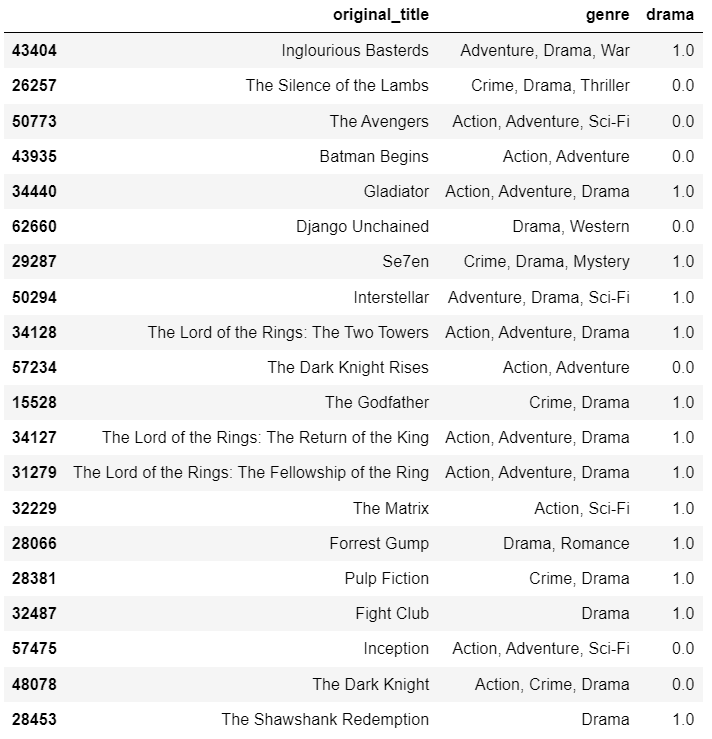
\includegraphics[scale = 1]{2_1}
        
    Ошибки есть, но в целом классификация верная

    \hypertarget{ux436ux430ux43dux440-ux43aux43eux43cux435ux434ux438ux44f}{%
\subsection{Жанр
комедия}\label{ux436ux430ux43dux440-ux43aux43eux43cux435ux434ux438ux44f}}

    \begin{tcolorbox}[breakable, size=fbox, boxrule=1pt, pad at break*=1mm,colback=cellbackground, colframe=cellborder]
\prompt{In}{incolor}{28}{\boxspacing}
\begin{Verbatim}[commandchars=\\\{\}]
\PY{k+kn}{from} \PY{n+nn}{sklearn}\PY{n+nn}{.}\PY{n+nn}{model\PYZus{}selection} \PY{k+kn}{import} \PY{n}{train\PYZus{}test\PYZus{}split}
\PY{n}{X} \PY{o}{=} \PY{n}{movies}\PY{p}{[}\PY{l+s+s1}{\PYZsq{}}\PY{l+s+s1}{description}\PY{l+s+s1}{\PYZsq{}}\PY{p}{]} \PY{o}{+} \PY{l+s+s1}{\PYZsq{}}\PY{l+s+s1}{ }\PY{l+s+s1}{\PYZsq{}} \PY{o}{+} \PY{n}{movies}\PY{p}{[}\PY{l+s+s1}{\PYZsq{}}\PY{l+s+s1}{actors}\PY{l+s+s1}{\PYZsq{}}\PY{p}{]} \PY{o}{+} \PY{l+s+s1}{\PYZsq{}}\PY{l+s+s1}{ }\PY{l+s+s1}{\PYZsq{}} \PY{o}{+} \PY{n}{movies}\PY{p}{[}\PY{l+s+s1}{\PYZsq{}}\PY{l+s+s1}{original\PYZus{}title}\PY{l+s+s1}{\PYZsq{}}\PY{p}{]} \PY{o}{+} \PY{l+s+s1}{\PYZsq{}}\PY{l+s+s1}{ }\PY{l+s+s1}{\PYZsq{}} \PY{o}{+} \PY{n}{movies}\PY{p}{[}\PY{l+s+s1}{\PYZsq{}}\PY{l+s+s1}{director}\PY{l+s+s1}{\PYZsq{}}\PY{p}{]} \PY{o}{+} \PY{l+s+s1}{\PYZsq{}}\PY{l+s+s1}{ }\PY{l+s+s1}{\PYZsq{}} \PY{o}{+} \PY{n}{movies}\PY{p}{[}\PY{l+s+s1}{\PYZsq{}}\PY{l+s+s1}{writer}\PY{l+s+s1}{\PYZsq{}}\PY{p}{]} \PY{o}{+} \PY{l+s+s1}{\PYZsq{}}\PY{l+s+s1}{ }\PY{l+s+s1}{\PYZsq{}} \PY{o}{+} \PY{n}{movies}\PY{p}{[}\PY{l+s+s1}{\PYZsq{}}\PY{l+s+s1}{production\PYZus{}company}\PY{l+s+s1}{\PYZsq{}}\PY{p}{]}
\PY{n}{X\PYZus{}train}\PY{p}{,} \PY{n}{X\PYZus{}test}\PY{p}{,} \PY{n}{y\PYZus{}train}\PY{p}{,} \PY{n}{y\PYZus{}test} \PY{o}{=} \PY{n}{train\PYZus{}test\PYZus{}split}\PY{p}{(}\PY{n}{X}\PY{p}{,} \PY{n}{movies}\PY{p}{[}\PY{l+s+s1}{\PYZsq{}}\PY{l+s+s1}{comedy}\PY{l+s+s1}{\PYZsq{}}\PY{p}{]}\PY{p}{,}
                                                    \PY{n}{random\PYZus{}state}\PY{o}{=}\PY{l+m+mi}{123}\PY{p}{,} \PY{n}{shuffle}\PY{o}{=}\PY{k+kc}{True}\PY{p}{,} \PY{n}{test\PYZus{}size}\PY{o}{=}\PY{l+m+mf}{0.25}\PY{p}{)}
\PY{n}{X\PYZus{}train} \PY{o}{=} \PY{n}{np}\PY{o}{.}\PY{n}{array}\PY{p}{(}\PY{n}{X\PYZus{}train}\PY{p}{)}
\PY{n}{X\PYZus{}test} \PY{o}{=} \PY{n}{np}\PY{o}{.}\PY{n}{array}\PY{p}{(}\PY{n}{X\PYZus{}test}\PY{p}{)}
\PY{n}{y\PYZus{}train} \PY{o}{=} \PY{n}{np}\PY{o}{.}\PY{n}{array}\PY{p}{(}\PY{n}{y\PYZus{}train}\PY{p}{)}
\PY{n}{y\PYZus{}test} \PY{o}{=} \PY{n}{np}\PY{o}{.}\PY{n}{array}\PY{p}{(}\PY{n}{y\PYZus{}test}\PY{p}{)}

\PY{n+nb}{print}\PY{p}{(}\PY{l+s+sa}{f}\PY{l+s+s1}{\PYZsq{}}\PY{l+s+s1}{пример текста}\PY{l+s+se}{\PYZbs{}n}\PY{l+s+si}{\PYZob{}}\PY{n}{X\PYZus{}train}\PY{p}{[}\PY{l+m+mi}{0}\PY{p}{]}\PY{l+s+si}{\PYZcb{}}\PY{l+s+s1}{\PYZsq{}}\PY{p}{)}
\PY{n+nb}{print}\PY{p}{(}\PY{l+s+sa}{f}\PY{l+s+s1}{\PYZsq{}}\PY{l+s+se}{\PYZbs{}n}\PY{l+s+s1}{размеры выборок: }\PY{l+s+si}{\PYZob{}}\PY{n+nb}{len}\PY{p}{(}\PY{n}{X\PYZus{}train}\PY{p}{)}\PY{p}{,} \PY{n+nb}{len}\PY{p}{(}\PY{n}{X\PYZus{}test}\PY{p}{)}\PY{l+s+si}{\PYZcb{}}\PY{l+s+s1}{\PYZsq{}}\PY{p}{)}
\end{Verbatim}
\end{tcolorbox}

    \begin{Verbatim}[commandchars=\\\{\}]
пример текста
While on holiday in Rhodes, Athenian war hero Darios becomes involved in two
different plots to overthrow the tyrannical king, one from Rhodian patriots and
the other from sinister Phoenician agents. Rory Calhoun, Lea Massari, Georges
Marchal, Conrado San Martín, Ángel Aranda, Mabel Karr, Mimmo Palmara, Roberto
Camardiel, Alfio Caltabiano, George Rigaud, Yann Larvor, Carlo Tamberlani, Félix
Fernández, Ignazio Dolce, Antonio Casas Il colosso di Rodi Sergio Leone Ennio De
Concini, Sergio Leone Cine-Produzioni Associate

размеры выборок: (58788, 19596)
    \end{Verbatim}

    \hypertarget{ux432ux44bux431ux43eux440-ux432ux435ux441ux430-ux44dux442ux430ux43f-0}{%
\subsubsection{Выбор веса (этап
0)}\label{ux432ux44bux431ux43eux440-ux432ux435ux441ux430-ux44dux442ux430ux43f-0}}

    \begin{tcolorbox}[breakable, size=fbox, boxrule=1pt, pad at break*=1mm,colback=cellbackground, colframe=cellborder]
\prompt{In}{incolor}{29}{\boxspacing}
\begin{Verbatim}[commandchars=\\\{\}]
\PY{n}{par0} \PY{o}{=} \PY{p}{\PYZob{}}
    \PY{l+s+s1}{\PYZsq{}}\PY{l+s+s1}{n\PYZus{}neighbors}\PY{l+s+s1}{\PYZsq{}}\PY{p}{:} \PY{p}{[}\PY{n}{i} \PY{k}{for} \PY{n}{i} \PY{o+ow}{in} \PY{n+nb}{range}\PY{p}{(}\PY{l+m+mi}{1}\PY{p}{,} \PY{l+m+mi}{11}\PY{p}{)}\PY{p}{]}\PY{p}{,}
    \PY{l+s+s1}{\PYZsq{}}\PY{l+s+s1}{weights}\PY{l+s+s1}{\PYZsq{}}\PY{p}{:} \PY{p}{[}\PY{p}{(}\PY{l+s+s1}{\PYZsq{}}\PY{l+s+s1}{uniform}\PY{l+s+s1}{\PYZsq{}}\PY{p}{,} \PY{l+s+s1}{\PYZsq{}}\PY{l+s+s1}{uniform}\PY{l+s+s1}{\PYZsq{}}\PY{p}{)}\PY{p}{,} \PY{p}{(}\PY{l+s+s1}{\PYZsq{}}\PY{l+s+s1}{linear}\PY{l+s+s1}{\PYZsq{}}\PY{p}{,} \PY{n}{linear}\PY{p}{)}\PY{p}{,} \PY{p}{(}\PY{l+s+s1}{\PYZsq{}}\PY{l+s+s1}{my\PYZus{}exp}\PY{l+s+s1}{\PYZsq{}}\PY{p}{,} \PY{n}{my\PYZus{}exp}\PY{p}{)}\PY{p}{,} \PY{p}{(}\PY{l+s+s1}{\PYZsq{}}\PY{l+s+s1}{distance}\PY{l+s+s1}{\PYZsq{}}\PY{p}{,} \PY{l+s+s1}{\PYZsq{}}\PY{l+s+s1}{distance}\PY{l+s+s1}{\PYZsq{}}\PY{p}{)}\PY{p}{]}\PY{p}{,}
    \PY{l+s+s1}{\PYZsq{}}\PY{l+s+s1}{scores}\PY{l+s+s1}{\PYZsq{}}\PY{p}{:} \PY{p}{[}\PY{n}{recall\PYZus{}score}\PY{p}{]}
\PY{p}{\PYZcb{}}
\end{Verbatim}
\end{tcolorbox}

    \begin{tcolorbox}[breakable, size=fbox, boxrule=1pt, pad at break*=1mm,colback=cellbackground, colframe=cellborder]
\prompt{In}{incolor}{ }{\boxspacing}
\begin{Verbatim}[commandchars=\\\{\}]
\PY{n}{folds0} \PY{o}{=} \PY{n}{fold\PYZus{}split}\PY{p}{(}\PY{n+nb}{len}\PY{p}{(}\PY{n}{y\PYZus{}train}\PY{p}{)}\PY{p}{,} \PY{l+m+mi}{4}\PY{p}{)}
\PY{n}{score\PYZus{}train0} \PY{o}{=} \PY{n}{cv\PYZus{}score}\PY{p}{(}\PY{n}{X\PYZus{}train}\PY{p}{,} \PY{n}{y\PYZus{}train}\PY{p}{,} \PY{n}{par0}\PY{p}{,} \PY{n}{folds0}\PY{p}{,} \PY{n}{neighbors}\PY{o}{.}\PY{n}{KNeighborsClassifier}\PY{p}{)}
\end{Verbatim}
\end{tcolorbox}

    \begin{tcolorbox}[breakable, size=fbox, boxrule=1pt, pad at break*=1mm,colback=cellbackground, colframe=cellborder]
\prompt{In}{incolor}{19}{\boxspacing}
\begin{Verbatim}[commandchars=\\\{\}]
\PY{n}{n} \PY{o}{=} \PY{l+m+mi}{10}
\PY{n}{score\PYZus{}weights} \PY{o}{=} \PY{p}{\PYZob{}}\PY{l+s+s1}{\PYZsq{}}\PY{l+s+s1}{uniform}\PY{l+s+s1}{\PYZsq{}}\PY{p}{:} \PY{l+m+mi}{0}\PY{p}{,} \PY{l+s+s1}{\PYZsq{}}\PY{l+s+s1}{linear}\PY{l+s+s1}{\PYZsq{}}\PY{p}{:} \PY{l+m+mi}{0}\PY{p}{,} \PY{l+s+s1}{\PYZsq{}}\PY{l+s+s1}{my\PYZus{}exp}\PY{l+s+s1}{\PYZsq{}}\PY{p}{:} \PY{l+m+mi}{0}\PY{p}{,} \PY{l+s+s1}{\PYZsq{}}\PY{l+s+s1}{distance}\PY{l+s+s1}{\PYZsq{}}\PY{p}{:} \PY{l+m+mi}{0}\PY{p}{\PYZcb{}}
\PY{k}{for} \PY{n}{i} \PY{o+ow}{in} \PY{n}{score\PYZus{}train0}\PY{p}{[}\PY{l+m+mi}{0}\PY{p}{]}\PY{o}{.}\PY{n}{keys}\PY{p}{(}\PY{p}{)}\PY{p}{:}
    \PY{n}{score\PYZus{}weights}\PY{p}{[}\PY{n}{i}\PY{p}{[}\PY{l+m+mi}{1}\PY{p}{]}\PY{p}{]} \PY{o}{+}\PY{o}{=} \PY{n}{score\PYZus{}train0}\PY{p}{[}\PY{l+m+mi}{0}\PY{p}{]}\PY{p}{[}\PY{n}{i}\PY{p}{]} \PY{o}{/} \PY{n}{n}
\PY{n}{score\PYZus{}weights}
\end{Verbatim}
\end{tcolorbox}

            \begin{tcolorbox}[breakable, size=fbox, boxrule=.5pt, pad at break*=1mm, opacityfill=0]
\prompt{Out}{outcolor}{19}{\boxspacing}
\begin{Verbatim}[commandchars=\\\{\}]
\{'uniform': 0.4381890393976558,
 'linear': 0.5140844925609015,
 'my\_exp': 0.5629390075229098,
 'distance': 0.5093544166360856\}
\end{Verbatim}
\end{tcolorbox}
        
    Экспоненциально взвешенные веса оказались лучше, но их качество не
улучшается с ростом числа соседей.

Произведём обучение на большем числе соседей, взвешивая по расстоянию
(предположительно это улучшит качество)

    \hypertarget{ux432ux44bux431ux43eux440-ux43aux43eux43bux438ux447ux435ux441ux442ux432ux430-ux441ux43eux441ux435ux434ux435ux439-ux44dux442ux430ux43f-1}{%
\subsubsection{Выбор количества соседей (этап
1)}\label{ux432ux44bux431ux43eux440-ux43aux43eux43bux438ux447ux435ux441ux442ux432ux430-ux441ux43eux441ux435ux434ux435ux439-ux44dux442ux430ux43f-1}}

    \begin{tcolorbox}[breakable, size=fbox, boxrule=1pt, pad at break*=1mm,colback=cellbackground, colframe=cellborder]
\prompt{In}{incolor}{13}{\boxspacing}
\begin{Verbatim}[commandchars=\\\{\}]
\PY{n}{tf\PYZus{}idf} \PY{o}{=} \PY{n}{TfidfVectorizer}\PY{p}{(}\PY{n}{max\PYZus{}df}\PY{o}{=}\PY{l+m+mf}{0.8}\PY{p}{,} \PY{n}{min\PYZus{}df}\PY{o}{=}\PY{l+m+mi}{10}\PY{p}{,} \PY{n}{stop\PYZus{}words}\PY{o}{=}\PY{l+s+s1}{\PYZsq{}}\PY{l+s+s1}{english}\PY{l+s+s1}{\PYZsq{}}\PY{p}{)}
\PY{n}{par1} \PY{o}{=} \PY{p}{\PYZob{}}
    \PY{l+s+s1}{\PYZsq{}}\PY{l+s+s1}{n\PYZus{}neighbors}\PY{l+s+s1}{\PYZsq{}}\PY{p}{:} \PY{p}{[}\PY{n}{i} \PY{k}{for} \PY{n}{i} \PY{o+ow}{in} \PY{n+nb}{range}\PY{p}{(}\PY{l+m+mi}{1}\PY{p}{,} \PY{l+m+mi}{200}\PY{p}{,} \PY{l+m+mi}{10}\PY{p}{)}\PY{p}{]}\PY{p}{,}
    \PY{l+s+s1}{\PYZsq{}}\PY{l+s+s1}{weights}\PY{l+s+s1}{\PYZsq{}}\PY{p}{:} \PY{p}{[}\PY{p}{(}\PY{l+s+s1}{\PYZsq{}}\PY{l+s+s1}{distance}\PY{l+s+s1}{\PYZsq{}}\PY{p}{,} \PY{l+s+s1}{\PYZsq{}}\PY{l+s+s1}{distance}\PY{l+s+s1}{\PYZsq{}}\PY{p}{)}\PY{p}{]}\PY{p}{,}
    \PY{l+s+s1}{\PYZsq{}}\PY{l+s+s1}{scores}\PY{l+s+s1}{\PYZsq{}}\PY{p}{:} \PY{p}{[}\PY{n}{recall\PYZus{}score}\PY{p}{,} \PY{n}{accuracy\PYZus{}score}\PY{p}{]}
\PY{p}{\PYZcb{}}
\end{Verbatim}
\end{tcolorbox}

    \begin{tcolorbox}[breakable, size=fbox, boxrule=1pt, pad at break*=1mm,colback=cellbackground, colframe=cellborder]
\prompt{In}{incolor}{17}{\boxspacing}
\begin{Verbatim}[commandchars=\\\{\}]
\PY{n}{folds1} \PY{o}{=} \PY{n}{fold\PYZus{}split}\PY{p}{(}\PY{n+nb}{len}\PY{p}{(}\PY{n}{y\PYZus{}train}\PY{p}{)}\PY{p}{,} \PY{l+m+mi}{4}\PY{p}{)}
\PY{n}{score\PYZus{}train1} \PY{o}{=} \PY{n}{cv\PYZus{}score}\PY{p}{(}\PY{n}{X\PYZus{}train}\PY{p}{,} \PY{n}{y\PYZus{}train}\PY{p}{,} \PY{n}{par1}\PY{p}{,} \PY{n}{folds1}\PY{p}{,} \PY{n}{neighbors}\PY{o}{.}\PY{n}{KNeighborsClassifier}\PY{p}{)}
\end{Verbatim}
\end{tcolorbox}

    \begin{tcolorbox}[breakable, size=fbox, boxrule=1pt, pad at break*=1mm,colback=cellbackground, colframe=cellborder]
\prompt{In}{incolor}{18}{\boxspacing}
\begin{Verbatim}[commandchars=\\\{\}]
\PY{n}{plt}\PY{o}{.}\PY{n}{plot}\PY{p}{(}\PY{n}{par1}\PY{p}{[}\PY{l+s+s1}{\PYZsq{}}\PY{l+s+s1}{n\PYZus{}neighbors}\PY{l+s+s1}{\PYZsq{}}\PY{p}{]}\PY{p}{,} \PY{n+nb}{list}\PY{p}{(}\PY{n}{score\PYZus{}train1}\PY{p}{[}\PY{l+m+mi}{0}\PY{p}{]}\PY{o}{.}\PY{n}{values}\PY{p}{(}\PY{p}{)}\PY{p}{)}\PY{p}{)}
\PY{n}{plt}\PY{o}{.}\PY{n}{plot}\PY{p}{(}\PY{n}{par1}\PY{p}{[}\PY{l+s+s1}{\PYZsq{}}\PY{l+s+s1}{n\PYZus{}neighbors}\PY{l+s+s1}{\PYZsq{}}\PY{p}{]}\PY{p}{,} \PY{n+nb}{list}\PY{p}{(}\PY{n}{score\PYZus{}train1}\PY{p}{[}\PY{l+m+mi}{1}\PY{p}{]}\PY{o}{.}\PY{n}{values}\PY{p}{(}\PY{p}{)}\PY{p}{)}\PY{p}{)}
\PY{n}{plt}\PY{o}{.}\PY{n}{xlabel}\PY{p}{(}\PY{l+s+s2}{\PYZdq{}}\PY{l+s+s2}{neighbors}\PY{l+s+s2}{\PYZdq{}}\PY{p}{)}
\PY{n}{plt}\PY{o}{.}\PY{n}{ylabel}\PY{p}{(}\PY{l+s+s2}{\PYZdq{}}\PY{l+s+s2}{score}\PY{l+s+s2}{\PYZdq{}}\PY{p}{)}
\end{Verbatim}
\end{tcolorbox}

            \begin{tcolorbox}[breakable, size=fbox, boxrule=.5pt, pad at break*=1mm, opacityfill=0]
\prompt{Out}{outcolor}{18}{\boxspacing}
\begin{Verbatim}[commandchars=\\\{\}]
Text(0, 0.5, 'score')
\end{Verbatim}
\end{tcolorbox}
        
    \begin{center}
    \adjustimage{max size={0.9\linewidth}{0.9\paperheight}}{output_61_1.png}
    \end{center}
    { \hspace*{\fill} \\}
    
    Предположение не оправдалось. Увеличение числа соседей при взвешивании
по расстоянию только снизило качество, остановимся на экспоненциальных в
случае комедии.

    \hypertarget{ux43eux431ux443ux447ux435ux43dux438ux435-ux43dux430-ux43bux443ux447ux448ux438ux445-ux43fux430ux440ux430ux43cux435ux442ux440ux430ux445}{%
\subsubsection{Обучение на лучших
параметрах}\label{ux43eux431ux443ux447ux435ux43dux438ux435-ux43dux430-ux43bux443ux447ux448ux438ux445-ux43fux430ux440ux430ux43cux435ux442ux440ux430ux445}}

    \begin{tcolorbox}[breakable, size=fbox, boxrule=1pt, pad at break*=1mm,colback=cellbackground, colframe=cellborder]
\prompt{In}{incolor}{25}{\boxspacing}
\begin{Verbatim}[commandchars=\\\{\}]
\PY{n}{neigh} \PY{o}{=} \PY{n}{neighbors}\PY{o}{.}\PY{n}{KNeighborsClassifier}\PY{p}{(}\PY{n}{n\PYZus{}neighbors}\PY{o}{=}\PY{l+m+mi}{5}\PY{p}{,} 
                                      \PY{n}{metric}\PY{o}{=}\PY{l+s+s1}{\PYZsq{}}\PY{l+s+s1}{cosine}\PY{l+s+s1}{\PYZsq{}}\PY{p}{,} \PY{n}{weights}\PY{o}{=}\PY{n}{my\PYZus{}exp}\PY{p}{)}
\PY{n}{scaler} \PY{o}{=} \PY{n}{TfidfVectorizer}\PY{p}{(}\PY{n}{max\PYZus{}df}\PY{o}{=}\PY{l+m+mf}{0.8}\PY{p}{,} \PY{n}{min\PYZus{}df}\PY{o}{=}\PY{l+m+mi}{10}\PY{p}{,} \PY{n}{stop\PYZus{}words}\PY{o}{=}\PY{l+s+s1}{\PYZsq{}}\PY{l+s+s1}{english}\PY{l+s+s1}{\PYZsq{}}\PY{p}{)}
\PY{n}{scaler}\PY{o}{.}\PY{n}{fit}\PY{p}{(}\PY{n}{X\PYZus{}train}\PY{p}{)}
\PY{n}{X\PYZus{}train} \PY{o}{=} \PY{n}{scaler}\PY{o}{.}\PY{n}{transform}\PY{p}{(}\PY{n}{X\PYZus{}train}\PY{p}{)}
\PY{n}{X\PYZus{}test} \PY{o}{=} \PY{n}{scaler}\PY{o}{.}\PY{n}{transform}\PY{p}{(}\PY{n}{X\PYZus{}test}\PY{p}{)}
\PY{n}{neigh}\PY{o}{.}\PY{n}{fit}\PY{p}{(}\PY{n}{X\PYZus{}train}\PY{p}{,} \PY{n}{y\PYZus{}train}\PY{p}{)}
\PY{n}{score\PYZus{}test1\PYZus{}acc} \PY{o}{=} \PY{n}{accuracy\PYZus{}score}\PY{p}{(}\PY{n}{y\PYZus{}test}\PY{p}{,} \PY{n}{neigh}\PY{o}{.}\PY{n}{predict}\PY{p}{(}\PY{n}{X\PYZus{}test}\PY{p}{)}\PY{p}{)}
\PY{n}{score\PYZus{}test1\PYZus{}rec} \PY{o}{=} \PY{n}{recall\PYZus{}score}\PY{p}{(}\PY{n}{y\PYZus{}test}\PY{p}{,} \PY{n}{neigh}\PY{o}{.}\PY{n}{predict}\PY{p}{(}\PY{n}{X\PYZus{}test}\PY{p}{)}\PY{p}{)}
\PY{n}{score\PYZus{}test1\PYZus{}acc}\PY{p}{,} \PY{n}{score\PYZus{}test1\PYZus{}rec}
\end{Verbatim}
\end{tcolorbox}

            \begin{tcolorbox}[breakable, size=fbox, boxrule=.5pt, pad at break*=1mm, opacityfill=0]
\prompt{Out}{outcolor}{25}{\boxspacing}
\begin{Verbatim}[commandchars=\\\{\}]
(0.6887119820371504, 0.5811213838353713)
\end{Verbatim}
\end{tcolorbox}
        
    \begin{tcolorbox}[breakable, size=fbox, boxrule=1pt, pad at break*=1mm,colback=cellbackground, colframe=cellborder]
\prompt{In}{incolor}{33}{\boxspacing}
\begin{Verbatim}[commandchars=\\\{\}]
\PY{n}{movies}\PY{p}{[}\PY{l+s+s1}{\PYZsq{}}\PY{l+s+s1}{drama}\PY{l+s+s1}{\PYZsq{}}\PY{p}{]}\PY{o}{.}\PY{n}{value\PYZus{}counts}\PY{p}{(}\PY{p}{)}
\end{Verbatim}
\end{tcolorbox}

            \begin{tcolorbox}[breakable, size=fbox, boxrule=.5pt, pad at break*=1mm, opacityfill=0]
\prompt{Out}{outcolor}{33}{\boxspacing}
\begin{Verbatim}[commandchars=\\\{\}]
1.0    43326
0.0    35058
Name: drama, dtype: int64
\end{Verbatim}
\end{tcolorbox}
        
    \begin{tcolorbox}[breakable, size=fbox, boxrule=1pt, pad at break*=1mm,colback=cellbackground, colframe=cellborder]
\prompt{In}{incolor}{34}{\boxspacing}
\begin{Verbatim}[commandchars=\\\{\}]
\PY{n}{movies}\PY{p}{[}\PY{l+s+s1}{\PYZsq{}}\PY{l+s+s1}{comedy}\PY{l+s+s1}{\PYZsq{}}\PY{p}{]}\PY{o}{.}\PY{n}{value\PYZus{}counts}\PY{p}{(}\PY{p}{)}
\end{Verbatim}
\end{tcolorbox}

            \begin{tcolorbox}[breakable, size=fbox, boxrule=.5pt, pad at break*=1mm, opacityfill=0]
\prompt{Out}{outcolor}{34}{\boxspacing}
\begin{Verbatim}[commandchars=\\\{\}]
0.0    51877
1.0    26507
Name: comedy, dtype: int64
\end{Verbatim}
\end{tcolorbox}
        
    Класс комедийных фильмов в два раза меньше некомедийных. Это могло
повлечь снижение качества recall


    % Add a bibliography block to the postdoc
    
 }

\newpage

\begin{flushleft}
\textbf{\section{Список литературы}}
\end{flushleft}

[1] Trevor Hastie, Robert Tibshirani, Jerome Friedman. "The elements of statistical learning: data mining, inference and prediction" — New York: Springer, 2017

[2] Журавлев Ю. И., Рязанов В. В., Сенько О. В. «Распознавание». Математические методы. Программная система. Практические применения. — М.: Фазис, 2006.

[3] Курс лекций по машинному обучению К.В. Воронцов 
\scriptsize http://www.machinelearning.ru/wiki/index.php?title=Машинное\_обучение\_\%28курс\_лекций\%2C\_К.В.Воронцов\%29




\end{document}